\documentclass[aps,prx,10pt,twocolumn,amsmath,amssymb,superscriptaddress]{revtex4-2}
\usepackage{graphicx} %include figure files
\usepackage{bm} %bold math
\usepackage{hyperref}% add hypertext capabilities
\usepackage{braket,bbold,color}

\usepackage[left=2cm,right=2cm,top=2cm,bottom=3cm]{geometry}
\usepackage{graphicx}
\usepackage{amsfonts}
\usepackage{amsmath}
\usepackage{mathtools}

\usepackage[english]{babel}

\def\UrlBreaks{\do\/\do-}

\usepackage{enumerate} % for numbering with [a)] format 

\DeclareUnicodeCharacter{0308}{}

\usepackage{amsthm}
\usepackage{float}

\newcommand{\cdag}{c^{\dag}}
\newcommand{\sgn}{\text{sgn}}
\newcommand{\ptot}{p_{\mathrm{tot}}}
\newcommand{\Hint}{H_{\mathrm{int}}}
\newcommand{\groundstate}{|\Omega\rangle}
\newcommand{\Mod}[1]{\ (\mathrm{mod}\ #1)}

\newcommand\scalemath[2]{\scalebox{#1}{\mbox{\ensuremath{\displaystyle #2}}}}

\theoremstyle{definition}
\newtheorem{definition}{Definition}[section]

\theoremstyle{definition}
\newtheorem*{example}{Example}

\newtheorem{theorem}{Theorem}
\newtheorem{lemma}[theorem]{Lemma}
\newtheorem{conjecture}{Conjecture}
\newtheorem{corollary}{Corollary}

\usepackage{amsmath}
%\usepackage{stmaryrd}

\bibliographystyle{apsrev4-2}

\newcommand{\blue}[1]{{\textcolor{blue}{#1}}}
\newcommand{\bs}[1]{\boldsymbol{#1}}

\widowpenalty10000
\clubpenalty10000

\begin{document}

\title{Hilbert Space Fragmentation in the Chiral Luttinger Liquid}

\author{Alexandre Chaduteau}
\affiliation{Blackett Laboratory, Imperial College London, London SW7 2AZ, United Kingdom}

\author{Nyan Raess}
\affiliation{Blackett Laboratory, Imperial College London, London SW7 2AZ, United Kingdom}

\author{Henry Davenport}
\affiliation{Blackett Laboratory, Imperial College London, London SW7 2AZ, United Kingdom}

\author{Frank Schindler}
\affiliation{Blackett Laboratory, Imperial College London, London SW7 2AZ, United Kingdom}

\begin{abstract}
The chiral Luttinger liquid develops quantum chaos as soon as a -- however slight -- nonlinear dispersion is introduced for the microscopic electronic degrees of freedom. For this nonlinear version of the model, we identify an infinite family of translation-invariant interaction potentials that display increasing degrees of Hilbert space fragmentation.
We corroborate this result by studying entanglement entropy and level statistics. We also develop a systematic understanding of the unconventional symmetries giving rise to fragmentation and use them to classify the possible fragmentation patterns. In particular, this approach allows us to predict the analytic block sizes and derive asymptotic scaling laws in the limit of large total momentum.
\end{abstract}

\maketitle

\section{Introduction} \label{sec: intro}
Classical thermalisation is a well-understood process; the analog for quantum systems has proven more subtle. Quantum non-ergodic/non-thermal systems have gathered much recent experimental and theoretical interest~\cite{Moudgalya_2022, Serbyn_2021, Bernien_2017, Zhang_2022, Larson_2013, Nandkishore_2015, experimental1, experimental2, experimental3}. Well-known quantum non-ergodic systems are integrable~\cite{Kitaev_2003,faddeev1996algebraic, Slavnov_2007} and putative many-body localised systems~\cite{Abanin_2019, alet2018many, pal2010many, abanin2017recent, Imbrie_2017}, which possess a large number of conserved quantities that prevent thermalisation altogether. Ergodicity breaking without the extensive number of conserved quantities has been found in systems displaying quantum many-body scarring~\cite{turner2018weak, papic2021weak, Yao_2022, MondragonShem_2021, Gotta_2023, PhysRevLett.122.173401, PhysRevB.101.195131, PhysRevB.101.205107, PhysRevResearch.2.022065, PhysRevResearch.2.043305, PhysRevB.98.155134, PhysRevB.104.L121103, PhysRevB.98.235156, PhysRevB.101.174308, PhysRevLett.125.230602, PhysRevResearch.1.033144, PhysRevB.102.085140, liska2023holographic}. Such systems possess a small number of Hamiltonian eigenstates, called quantum many-body scars (QMBS), which do not thermalise. Although exceptions have been found~\cite{Langlett_2022, PhysRevLett.127.150601}, these isolated scar states characteristically display lower real-space entanglement entropy scaling than thermal states. In addition to this, dipole-conserving Hamiltonians~\cite{First_HSF_2020} recently provided the first example of systems whose whole Hilbert space splits/fragments into dynamically disconnected subspaces~\cite{PhysRevX.12.011050, SciPostPhys.13.4.098, HSF_opensystems, PhysRevB.103.235133, Brighi_2023, PhysRevE.104.044106}. This phenomenon is now called Hilbert Space Fragmentation (HSF)~\cite{Moudgalya_2022} (or simply fragmentation) and can be regarded as a generalisation of QMBS.

We study the chiral non-linear Luttinger liquid (CNLLL)~\cite{Haldane_1981, 1.1342524, doi:10.1126/science.1165403, RevModPhys.75.1449, SIRKER_2012}, a 1D model of interacting fermions with non-linear but unidirectional dispersion. This is a paradigmatic model within condensed matter physics that has two well-known integrable limits: (1) a free fermion limit where the fermion-fermion interaction is removed and (2) a free boson limit where the dispersion relation is linear~\cite{Haldane_1981}. Non-linear terms in the dispersion relation however make the model non-integrable. Recent work~\cite{Schindler_2022} uncovered families of exact Hamiltonian eigenstates in the CNLLL, for certain choices of the fermion-fermion interaction potential. These exact states share a core property of QMBS~\cite{IvarMartinLLScars22}, in that they have characteristically lower entanglement entropy compared to other eigenstates, when subdividing the system in \emph{momentum space}.

Here we uncover an infinite family of interaction potential configurations that produce HSF in the CNLLL, thus generalising the isolated scars of Ref.~\onlinecite{Schindler_2022}. To study fragmentation in the CNLLL, we compute each Hilbert subspace's momentum-space entanglement entropies and level statistics. As is typical of fragmented systems, each Hilbert subspace presents its own `band' of entropies in the entanglement spectrum. We obtain a simple positive integer parameter, $n$, that generates different realisations of the CNLLL with varying levels of fragmentation. As $n$ increases (with other parameters fixed), the corresponding system becomes increasingly fragmented, until each eigenstate of the Hamiltonian forms its own disconnected Hilbert subspace. We find explicit relations for the block sizes and show that, at least in some cases, the fragmentation pattern can be predicted analytically.

We should note that there are varying definitions of HSF used in the literature; for example, that the number of Hamiltonian blocks should scale exponentially rather than polynomially in the system size $L$~\cite{PhysRevX.12.011050}. In our case, this definition is difficult to apply: the CNLLL is a continuum system, and a finite Hilbert space is not obtained by fixing the system size $L$, but instead by fixing the total momentum $\ptot$. While the number of blocks we find in this work scales polynomially in $\ptot$, we use the label HSF because: (1) the fraction of Hilbert space occupied by the largest block approaches zero in the limit $\ptot \rightarrow \infty$, and (2) the blocks are labelled by eigenvalues of highly \emph{non-local} symmetry operators, which can be viewed as momentum-space modulated symmetries~\cite{Sala22modulated}. (We also note that some examples of HSF with polynomial scaling in $L$ are known~\cite{Arijeet22weakfragmentation}.)

The paper is organised as follows. The necessary background on the CNLLL is given in Sec.~\ref{sec:background}. In Sec.~\ref{sec:fragpatterns} we introduce the basic mechanism for HSF and discuss the unconventional symmetry operators whose eigenvalues resolve the fragments. In Sec.~\ref{sec:entropyandlvlstats} we study the thermal structure of the fragmented Hamiltonians such as the entanglement entropy and the energy level statistics. Lengthy proofs and more detailed numerics are relegated to the appendices.

\section{Model} \label{sec:background}
The Luttinger liquid is a 1D model of interacting fermions, defined here on a circle of circumference $L$. We take the operator $c_{x}$ to annihilate a spinless electron at position $x$ where $x \in [0, L)$. Then
\begin{equation}
   \begin{aligned}
   &\{c_x, \cdag_y\} = \delta(x-y), \;\;\; \{c_x, c_y\} = \{\cdag_x, \cdag_y\} = 0, \\
   &\{c_p, \cdag_q\} = \delta_{pq}, \;\;\;\;\;\;\;\;\;\;\;\; \{c_p, c_q\} = \{\cdag_p, \cdag_q\} = 0,
   \end{aligned}
\end{equation}
where the momentum space ($p$) and real space ($x$) operators are related by Fourier transforms,
\begin{equation}
\cdag_p = \frac{1}{\sqrt{L}}\int_{-L/2}^{L/2} \mathrm{d} x \, e^{\mathrm{i} px}\cdag_x, \;\;\; \cdag_x = \frac{1}{\sqrt{L}}\sum_p e^{-\mathrm{i} px}\cdag_p,
\end{equation}
and $p \in \frac{2\pi}{L}\mathbb{Z}$ due to periodic boundary conditions. \textbf{We set $\bs{L = 2\pi}$ from now on} so that all momenta are integers.
The Luttinger liquid Hamiltonian splits into a kinetic ($H_{\mathrm{kin}}$) and fermion-fermion interaction part ($H_{\mathrm{int}}$),
\begin{equation} \label{eq: basic hamiltonian def}
H = H_{\mathrm{kin}} + H_{\mathrm{int}},
\end{equation}
where
\begin{equation}
   \begin{aligned}
& H_{\mathrm{kin}} = \sum_{p}\epsilon(p)\cdag_pc_p, \\
& H_{\mathrm{int}} = \int_{-L/2}^{L/2} \mathrm{d} x\int_{-L/2}^{L/2} \mathrm{d} y \, V(x-y) \, \cdag_xc_x\cdag_yc_y.
   \end{aligned}
\end{equation}
$H_{\mathrm{int}}$ encodes a two-body interaction with a translationally-invariant potential $V(x, y) = V(x-y)$, which could be e.g. of the Coulomb form. We only consider inversion-symmetric potentials i.e. $V(x) = V(-x)$. To guarantee chirality, we assume that the dispersion relation $\epsilon(p)$ obeys the condition $\sgn[\epsilon(p)] = \sgn(p)$ for all momenta $|p| \ll \Lambda$, where $\Lambda$ is a momentum cut-off scale, usually given by a microscopic lattice spacing $d$ as $\Lambda \sim 1/d$. For instance, Eq.~\eqref{eq: basic hamiltonian def} could be the effective low-energy Hamiltonian governing the 1D chiral edge mode of a 2D Chern insulator with Chern number $C = 1$, microscopically defined on a lattice with spacing $d$.

In momentum space, the many-body ground state $\groundstate = \prod_{p \leq 0} c^\dagger_p \ket{0}$ of $H_{\mathrm{kin}}$ has all momenta with non-positive $\epsilon(p)$ occupied ($\ket{0}$ is the absolute fermionic vacuum). To make the theory well-defined, we normal-order ($:\mathrel{\ }:$) all operators $\mathcal{O}$ such that 
$
:\mathrel{\mathcal{O}}: = \mathcal{O} - \langle \Omega | \mathcal{O} | \Omega \rangle.
$
This shifts the kinetic energy of $\groundstate$ to zero and allows us to take the limit $\Lambda \rightarrow \infty$ without divergences.

\begin{figure}[t]
  \centering
  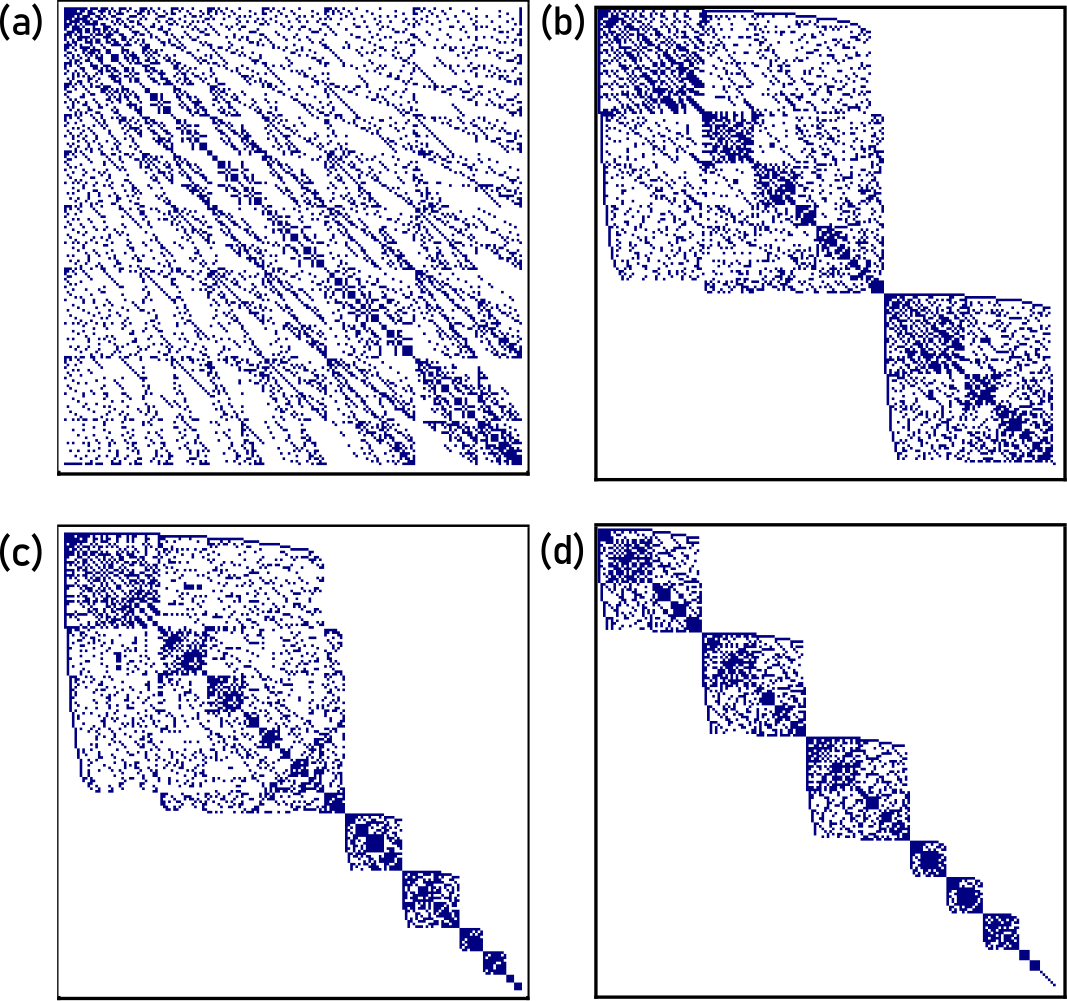
\includegraphics[scale=0.48, width = \columnwidth]{figures/ptot15_p1p2p3p4_patterns_png.png}
  \caption{Fermionic basis matrix representations of $:\mathrel{\Hint}:$ for $\ptot = 15$; $v = 1$, $a = 0.1/\ptot$ in $\epsilon(p)=v p + a p^2$.  Fragmentation patterns corresponding to different unconventional symmetries $T_n$ [Eq.~\eqref{eq: symmetry def}] are shown; white and navy pixels represent zero and non-zero matrix elements respectively. The Hilbert space dimension is given by the number of partitions $\mathcal{P}(15) = 176$. (a) $T_1$: No constraints are enforced on the interaction potentials $V_p$ and so the matrix does not block-diagonalise. (b) $T_2$: every potential $V_p$ with $p$ odd is set equal and the matrix splits in two blocks. (c) $T_3$: every potential with $p$ not a multiple of $3$ is set equal. (d) $T_4$: every potential with $p$ not a multiple of $4$ is set equal. In all cases, $V(p) = 0.1$ for all Fourier modes included in the pattern $P_n$, otherwise they are randomly drawn from the interval $[0.05, 0.15]$.}
\label{fig:matrices}
\end{figure}

The Luttinger Hamiltonian in Eq.~\eqref{eq: basic hamiltonian def} has two important conventional symmetries: (1) $U(1)$ phase rotation symmetry, with an associated conserved total particle number $N = \sum_p \cdag_p c_p$, and (2) spatial translation symmetry, with conserved total momentum $P = \sum_p p \cdag_p c_p$. When normal-ordering, $:\mathrel{N}:\groundstate = 0$ and $:\mathrel{P}:\groundstate = 0$. \newline
\textbf{From now on, we work within the charge-neutral Hilbert space sector of} $\bs{\langle:\mathrel{N}:\rangle = 0}$. Also, since total momentum is conserved, we can work within a sector of fixed total momentum $\langle :\mathrel{P}:\rangle = \ptot$. 

The full Hilbert space is spanned by basis states of the form 
\begin{equation}
|\textbf{n}, \bar{\textbf{n}}\rangle = \prod_{p>0}c^{\dag n_p}_p \prod_{p\leq 0}c^{\bar{n}_p}_p \;\groundstate,
\label{eq:ferm_basis}
\end{equation}
where $\textbf{n}$ and $\bar{{\textbf{n}}}$ are particle/hole occupation vectors, with entries equal to $0$ or $1$. Since $:\mathrel{N}:\groundstate = 0$, both $\textbf{n}$ and $\bar{{\textbf{n}}}$ have the same number of non-zero entries. We will use this basis exclusively, and sometimes refer to it as the \emph{fermionic basis}, to distinguish it from the more commonly used bosonic basis for the linear Luttinger liquid~\cite{Haldane_1981}. While the bosonic basis diagonalises both $H_{\mathrm{kin}}$ and $H_{\mathrm{int}}$ of the linear Luttinger liquid where $\epsilon(p) \sim p$, it does not diagonalize the CNLLL where $\epsilon(p) = v p + a p^2 + \dots$, because in this case $H_{\mathrm{kin}}$ becomes non-diagonal in the bosonic basis. For our purposes, it is easier to work with the fermionic basis, at least as long as we do not restrict to a specific form of the nonlinear dispersion $\epsilon(p)$. Ordering these states by their total momentum eigenvalue, the dimension of the sector with $\langle :\mathrel{N}: \rangle = 0$, $\langle :\mathrel{P}: \rangle = \ptot$ is $\mathcal{P}(\ptot)$, the number of integer partitions of $\ptot$ \cite{Haldane_1981, Wright_1965}.

The normal-ordered interaction Hamiltonian $:\mathrel{\Hint}:$ can be simplified as~\cite{Schindler_2022}
\begin{equation} \label{eq:hint}
\begin{aligned}
&:\mathrel{\Hint}: = \\ &\sum_{q>k}\sum_{p>(k-q)/2}\biggl[V(q-k+p) - \delta_{p \neq 0}V(|p|)\biggr]\cdag_{q+p}c_q c_k \cdag_{k-p},
\end{aligned}
\end{equation}
where
$
    V(p) = \frac{1}{L}\int \mathrm{d} x \, e^{ipx}V(x)
$
is the Fourier transform of the real-space potential.
This form of the Hamiltonian will turn out to be most useful form to investigate HSF.

In the non-interacting limit $V(x) = 0$, the eigenstates of the full Hamiltonian $:\mathrel{H}:$ have a simple form because the kinetic term ($:\mathrel{H_{\mathrm{kin}}}:$) is diagonal in momentum space. We label the eigenstates of $:\mathrel{H_{\mathrm{kin}}}:$ in each total momentum sector ($\ptot$) as $\ket{\phi_i}$. For example for $\ptot=3$ we have the three states
\begin{equation}
\ket{\phi_1} = c^\dagger_3 c_0 \ket{\Omega}, \quad \ket{\phi_2} = c^\dagger_2 c_{-1} \ket{\Omega}, \quad \ket{\phi_3} = c^\dagger_1 c_{-2} \ket{\Omega}. 
\label{eq:ptot3_states}
\end{equation}
To declutter the notation, \textbf{we will drop all normal ordering symbols ($:\mathrel{\ }:$) from now on}, and implicitly assume that all operators are properly normal-ordered.

\begin{figure}[t]
  \centering
  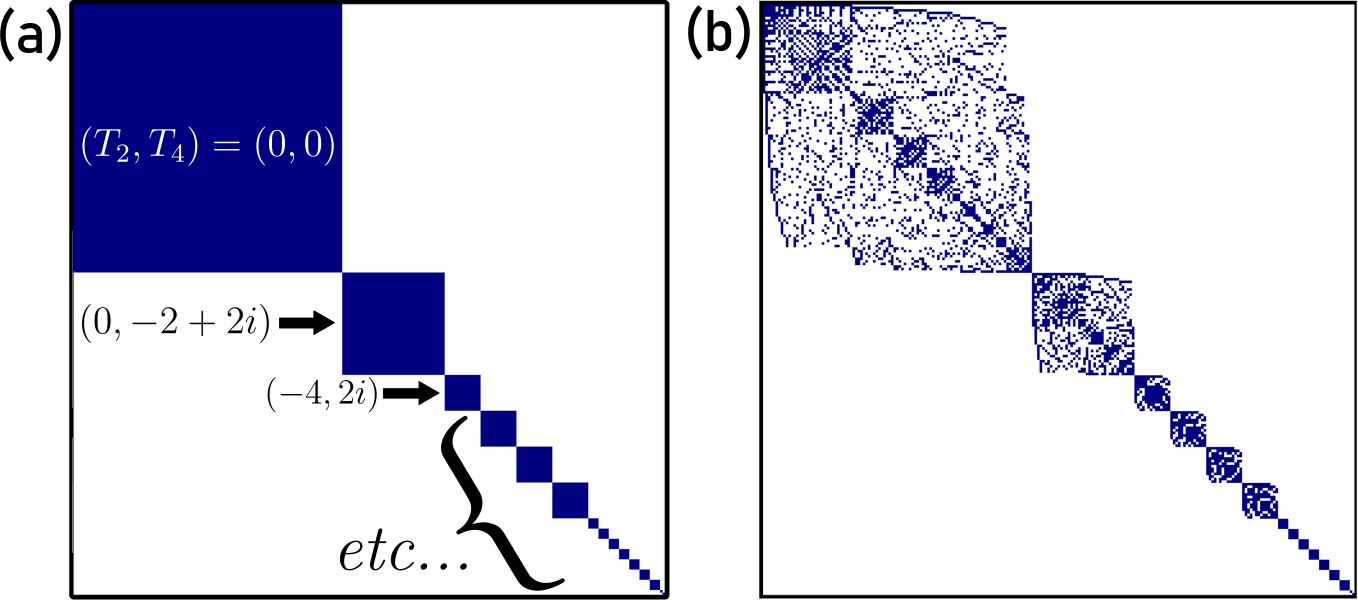
\includegraphics[scale=0.5, width = \columnwidth]{figures/analytical_vs_real_block_matrix_n_4_ptot_16_FINAL_navy_png.png}
  \caption{(a) Block pattern of ${H}$ for $\ptot = 16$ when grouping basis states by their set of eigenvalues of operators $(T_2, T_4)$. (b) Hamiltonian for $\ptot=16$ and the $P_4$ pattern, after block-diagonalisation. Numerical parametre values are the same as in Fig. \ref{fig:matrices}. We set $V(p) = 0.1$ for modes in the $P_4$ pattern; all other modes are drawn randomly from $[0.05, 0.15]$. The blocks in (a) and (b) match.}
\label{fig:analytical_vs_real_blocks}
\end{figure}

\begin{figure}[t]
  \centering
  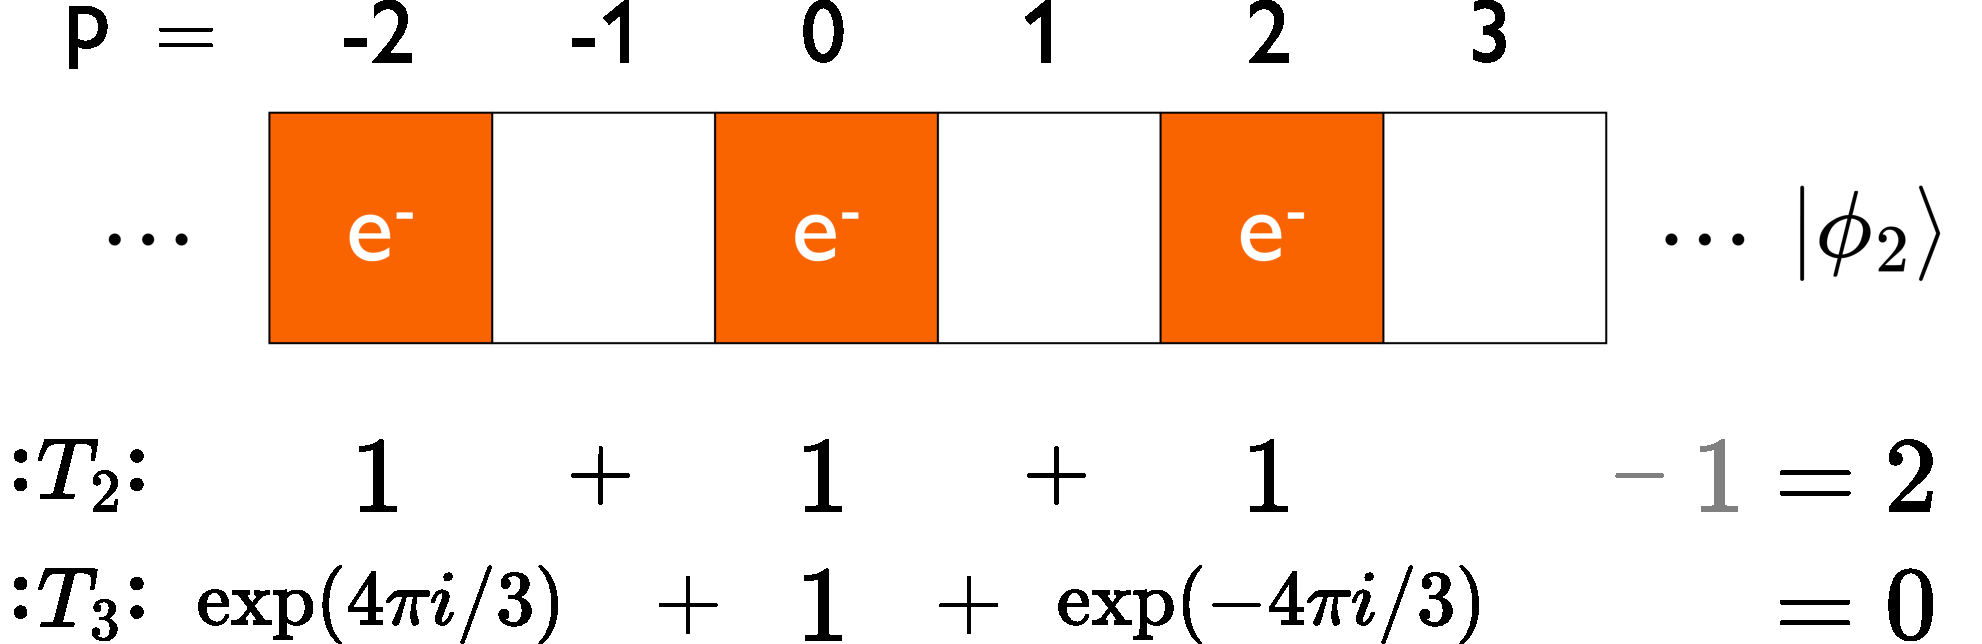
\includegraphics[scale=0.5, width = \columnwidth]{figures/eigenvalue_demo.pdf}
  \caption{Example calculation of $:\mathrel{T_2}:$ and $:\mathrel{T_3}:$ eigenvalues of the state $\ket{\phi_2} = c_2^{\dagger}c_{-1}\ket{\Omega}$ at $\ptot = 3$. Normal ordering leads to the extra $-1$ term in the $:\mathrel{T_2}:$ eigenvalue.}
\label{fig:eigval_demo}
\end{figure}

\section{Fragmentation Patterns}
\label{sec:fragpatterns}
Each realisation of the CNLLL requires specifying the nonlinear dispersion $\epsilon(p)$ as well as the Fourier components of the interaction potential $V(p)$. We define a family of potential patterns $V(p)$, where we \textbf{set equal} all elements in the set
\begin{equation}
P_n = \{V(p) \, | \, p \in [1, \ptot], \, p \notin n \mathbb{Z}\}.
\label{eq:potential_seq}
\end{equation}
For any choice of chiral dispersion $\epsilon(p)$, these choices of $V(p)$ result in HSF. For example, $P_2 = \{V(1), V(3), ... \}$ corresponds to setting all odd-momentum Fourier components equal. 

An example of the block-diagonal structure of the interaction Hamiltonian matrix elements $\braket{\phi_i | \Hint | \phi_j}$ for $V(p)$ observing $P_2$ and $P_3$ for $\ptot=15$ is shown in Fig. \ref{fig:matrices}. Note that there are more blocks for $P_3$ than $P_2$; this is because $P_3$ implies a larger number of constraints. In general, as $n$ increases, more and more blocks are produced at a given $\ptot$. This proceeds until the Hamiltonian becomes fully diagonal at $n = \ptot + 1$. The resulting blocks can be labelled by the eigenvalues of a family of unconventional symmetry operators that commute with the Hamiltonian.

\subsection{Symmetries}
\label{sec:symmetries}
For each potential tuning pattern $P_n$, there exist two (Hermitian) symmetry generators that commute with the full CNLLL Hamiltonian in Eq.~\eqref{eq: basic hamiltonian def}, defined by 
\begin{equation} \label{eq:sym_operators}
 \begin{gathered}
 T^{(1)}_n = \sum_{p} \cos{\left(\frac{2\pi}{n} p \right)} \cdag_{p}c_p, \\
 T^{(2)}_n = \sum_{p} \sin{\left(\frac{2\pi}{n} p \right)} \cdag_{p}c_p.
\end{gathered}
\end{equation}
We explicitly prove this statement in Appendix \ref{appendix:derivation}.
For example, $T^{(1)}_1 = N$ is the number operator and $T^{(2)}_1 = 0$. The first non-trivial operator is $T^{(1)}_2 = \sum_{p}(-1)^p \cdag_p c_p$ which counts $n_\mathrm{e} - n_\mathrm{o}$, the occupation number of even momenta states minus odd momenta states, while $T^{(2)}_2 = 0$ still only generates the identity. 
All fermionic states of the form (\ref{eq:ferm_basis}) are eigenstates of these symmetry operators.
It is practical to package these two operators into a single operator
\begin{equation} \label{eq: symmetry def}
T_n = \sum_{p}e^{\mathrm{i} \frac{2 \pi}{n} p}\cdag_p c_p,
\end{equation}
that is neither Hermitian nor unitary.
The Hamiltonian blocks are then labeled by the eigenvalues of ${T_n}$. In fact, given a set of $V(p)$'s observing $P_n$, not only does $T_n$ commute with ${H}$, but also $T_{f}$ for any integer factor $f$ of $n$. If $\{f_1, f_2...\}$ is the set of factors of $n$, then each block is uniquely identified by a set of eigenvalues $\{\lambda_{f_1}, \lambda_{f_2}...\}$, one for each operator $T_{f_i}$ (see Fig.~\ref{fig:analytical_vs_real_blocks} for an example).

\begin{figure}[t]
  \centering
  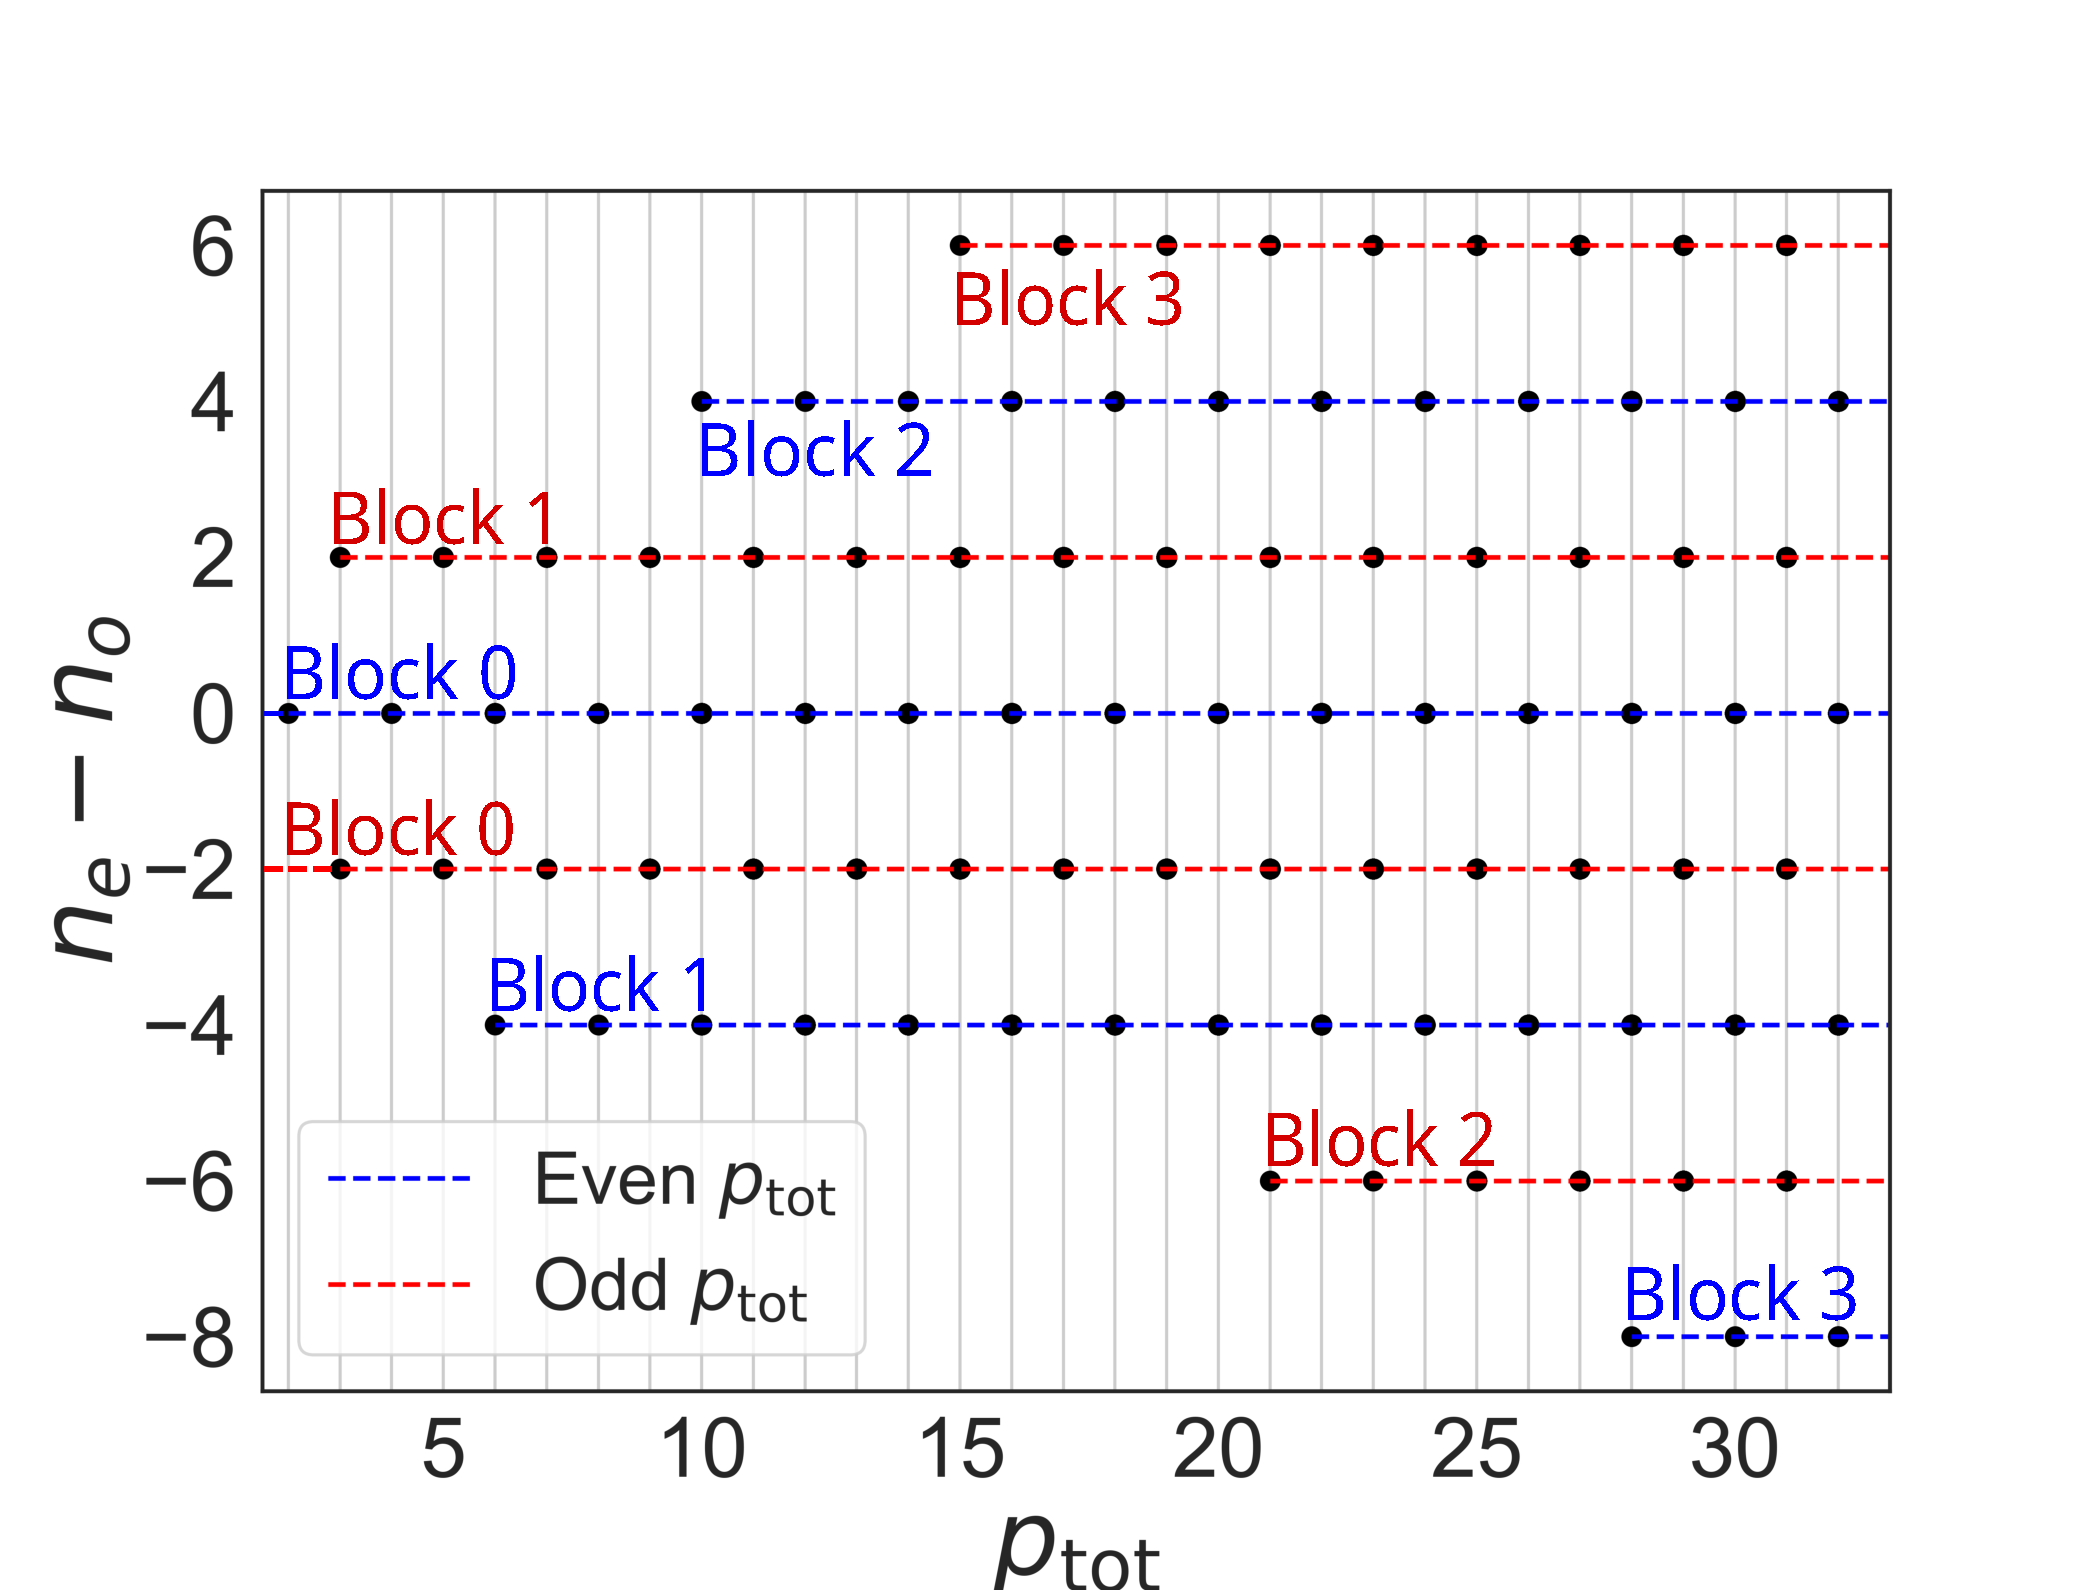
\includegraphics[scale=0.5, width = \columnwidth]{figures/even-odd_occ_REFINED.pdf}
  \caption{Fragmented blocks induced by the symmetry $T_2$ and their eigenvalues $n_\mathrm{e} - n_\mathrm{o}$ against $\ptot$. New blocks arise exactly at triangular numbers $t_i$ [Eq.~\eqref{eq:triang_nums}]. Note that there are families of blocks with the same eigenvalues for a range of $\ptot$ even (blue) and $\ptot$ odd (red).}
\label{fig:oddevenoccupancies}
\end{figure}

The eigenvalues of the $T_n$ operator are always some linear combination of the $n\text{-th}$ roots of unity; an example is given in Fig. \ref{fig:eigval_demo}. At $\ptot = 3$, the state $\ket{\phi_2} = c^\dagger_2 c_{-1} \ket{\Omega}$ from (\ref{eq:ptot3_states}) has $T_2$ eigenvalue 2, while $\ket{\phi_1}$ and $\ket{\phi_3}$ have eigenvalue $-2$. Correspondingly, when all $V(p)$ in $P_2$ are set equal [so that $V(1) = V(3) \neq V(2)$], only $\ket{\phi_1}$ and $\ket{\phi_3}$ interact with one another, while $\ket{\phi_2}$ remains as an isolated ``scar" state. As for $T_3$, since all three states have different $T_3$ eigenvalues, the matrix becomes diagonal when $P_3$ is enforced; all states are disconnected.

The number of different eigenvalues of $T_n$ that appear is dependent on the $\ptot$ subsector (see Fig.~\ref{fig:oddevenoccupancies}). For example, at $\ptot = 6$, the state $c_{-2}c_0c_1^{\dagger}c_3^{\dagger}\groundstate$ has $T_2$ eigenvalue $-4$, but at smaller total momenta there is no state with this eigenvalue. We say that this eigenvalue is `new' at $\ptot = 6$. More precisely, there is a `new' block at total momentum $p$ if the set of eigenvalues $\{\lambda_{f_1}, \lambda_{f_2}...\}$ that label it is not shared by any state in subsectors $\ptot < p$. Conversely, the remaining blocks can be uniquely identified with blocks appearing for smaller $\ptot$, as they share the same eigenvalues $\{\lambda_{f_1}, \lambda_{f_2}...\}$.

\begin{figure}[t]
  \centering
  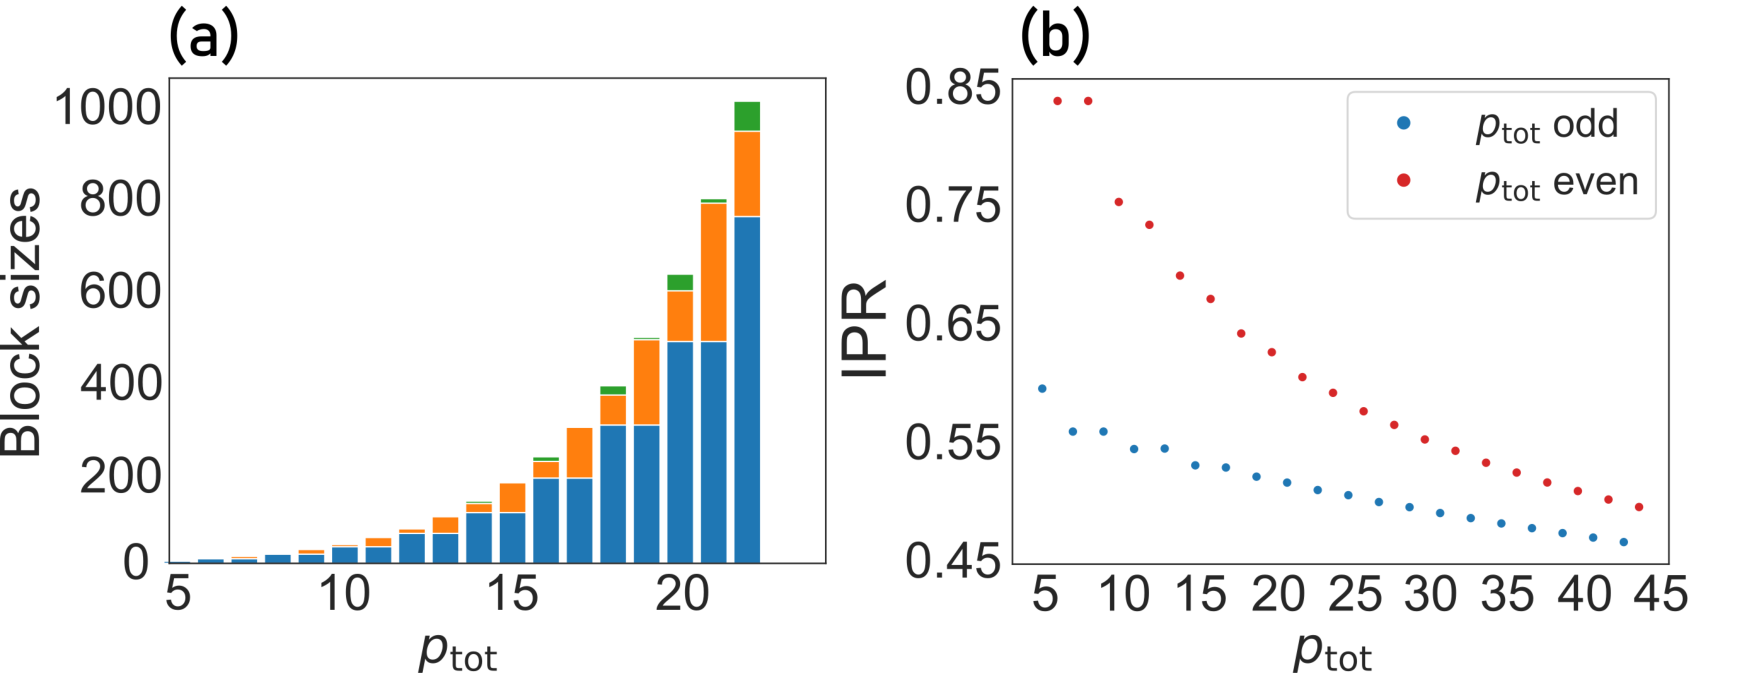
\includegraphics[width = 0.5\textwidth]{figures/blocks_and_iprs_n_2_BIGGER_again_png.pdf}
  \caption{(a) Stacked-bar histograms of block sizes of the Hamiltonian matrix at a given $\ptot$, for symmetry $T_2$. Each colour represents a different block; the height of a whole bar is the full Hilbert space dimension. (b) Inverse participation ratio [IPR, Eq.~\eqref{eq: ipr def}] of the block distribution against $\ptot$ for $P_2$. A high IPR implies a peaked distribution (only a few blocks dominate the full Hilbert space), while a low IPR implies a broad distribution (many blocks coexist with roughly similar sizes). We colour-code the $\ptot$ that are odd or even.}
\label{fig:blockpops}
\end{figure}

\subsection{Analytical results on block sizes}
\label{sec:block_pop_sizes}
For the sequence of symmetries $T_n$ with $n$ prime, our numerical results suggest that blocks `grow' according to the sequence $a_n(j)$, the number of partitions of $j$ into integers of $n$ kinds (for $n=2$, see Ref. \cite{OEIS_sequence}). For instance, $a_2(2)=5$ because, labelling the two kinds of integer as primed and unprimed, we have 
\begin{equation*}
    2 = 2' = 1+1 = 1'+1' = 1+1'
\end{equation*}
giving five possible partitions. If a block is `new' at $\ptot = p$, it will be of size $a_n(j)$ at $\ptot = p+nj$ (where $n$ is fixed by the assumption of symmetry $T_n$ and the statement holds for any choice of non-negative $j$). Since $a_n(0) \equiv 1$, a new block always consists of a single state; equivalently, at each $\ptot$ at which a new eigenvalue occurs, there is only one state with that eigenvalue. As a minimal example, take the symmetry $T_2$; the block with $T_2$ eigenvalue 0 begins at $\ptot = 0$ with only the ground state $\groundstate$, and at $\ptot = 4$ this block contains 5 states. The generating function of the sequence $a_n(j)$ is 
\begin{equation}
    z_n(x) = \prod_{k \geq 1}\frac{1}{(1-x^k)^n},
    \label{eq:generating_func}
\end{equation}
meaning that $z_n(x) = a_n (0) + a_n (1) \, x + a_n (2) \, x^2 + a_n (3) \, x^3 + \cdots$.
For the symmetry $T_2$ we give a proof that $a_2(j)$ calculates the block sizes in Appendix \ref{appendix:T2_example}. For $n\neq 2$ the above remains a conjecture to which we have not found a numerical counterexample for $n \leq 10$ and $\ptot \leq 30$. Numerically, we have observed that the series $a_n (j)$ also predicts block sizes for $n$ non-prime, i.e. even when further symmetries $T_f$ for all factors $f$ of $n$ are present. 

\begin{figure}[t]
  \centering
  \includegraphics[scale=0.5, width = \columnwidth]{figures/triangular_states.png}
  \caption{A triangular state at $\ptot = 10$. Any eigenvalue of the $T_2$ operator may be expressed as $\lambda = n_{\text{e}}-n_{\text{o}}$, where $n_{\text{e}}$ and $n_{\text{o}}$ denote the number of even and odd momentum sites occupied. To maximise $|\lambda|$ while minimising $\ptot$ one must remove the first available odd/even electron sites and replace them at even/odd sites. As shown above for the case $10 = 4+3+2+1$, this always results in a triangular number.}
\label{fig:triangular_states}
\end{figure}

Fig. \ref{fig:blockpops} shows the block populations for $T_2$, whose block sizes are predicted by sequence $a_2$. The number of blocks scales polynomially with $\ptot$. This should be contrasted with a definition of HSF where the number of blocks scales exponentially with the system size $L$~\cite{Moudgalya_2022}, see our discussion in Sec.~\ref{sec: intro}. We include a similar plot for $T_3$ in the Appendix, Fig.~\ref{fig:blockpops_n_3}.

For the symmetry $T_2$ we can also predict the values of $\ptot$ at which new Hamiltonian blocks arise: the $T_2$ operator gains a new eigenvalue (i.e. there is a new block) whenever $\ptot$ reaches a triangular number, where the triangular numbers, $t_i$, are defined as the sum of the first $i$ non-zero integers: 
\begin{equation} \label{eq:triang_nums}
    t_i = \sum_{k=1}^{i} k = \frac{i (i+1)}{2}.
\end{equation} We call the special state that has the new eigenvalue at $\ptot = t_i$ a \textit{triangular state} $\ket{\Delta_i}$, with eigenvalue $\Delta_i$. Fig. \ref{fig:oddevenoccupancies} shows new blocks arising at triangular numbers, as well as their associated eigenvalues. Any  eigenvalue that is new has the largest possible magnitude in its $\ptot$ subspace; we motivate this in Fig.~\ref{fig:triangular_states}. As $n$ increases new blocks quickly start to arise in almost every $\ptot$ sector.

Numerically, for $n=3$ blocks arise at numbers matching OEIS sequence A267137~\cite{OEIS_sequence_n_3} (apart from the second entry of the sequence, which could be considered an edge/convention issue). This observation could help in proving the conjecture for higher $n$.

Finally we note that our block size conjecture relates blocks at $\ptot$ with those at $\ptot + nj$; numerically, we know this is because, if $T_n$ has some set of eigenvalues $\{\lambda_{n_1}, \lambda_{n_2}, \lambda_{n_3}...\}$ labelling blocks in a $\ptot$ subsector, those eigenvalues will next appear in the $\ptot + n$ subsector (see Fig.~\ref{fig:oddevenoccupancies} for $T_2$ where eigenvalues reappear whenver $\ptot$ is advanced by $2$). This means we can consider each of the $n \ `\ptot \ \text{mod} \ n$' sequences separately (Appendix \ref{appendix:T2_example}).

\begin{figure}[t]
  \centering
  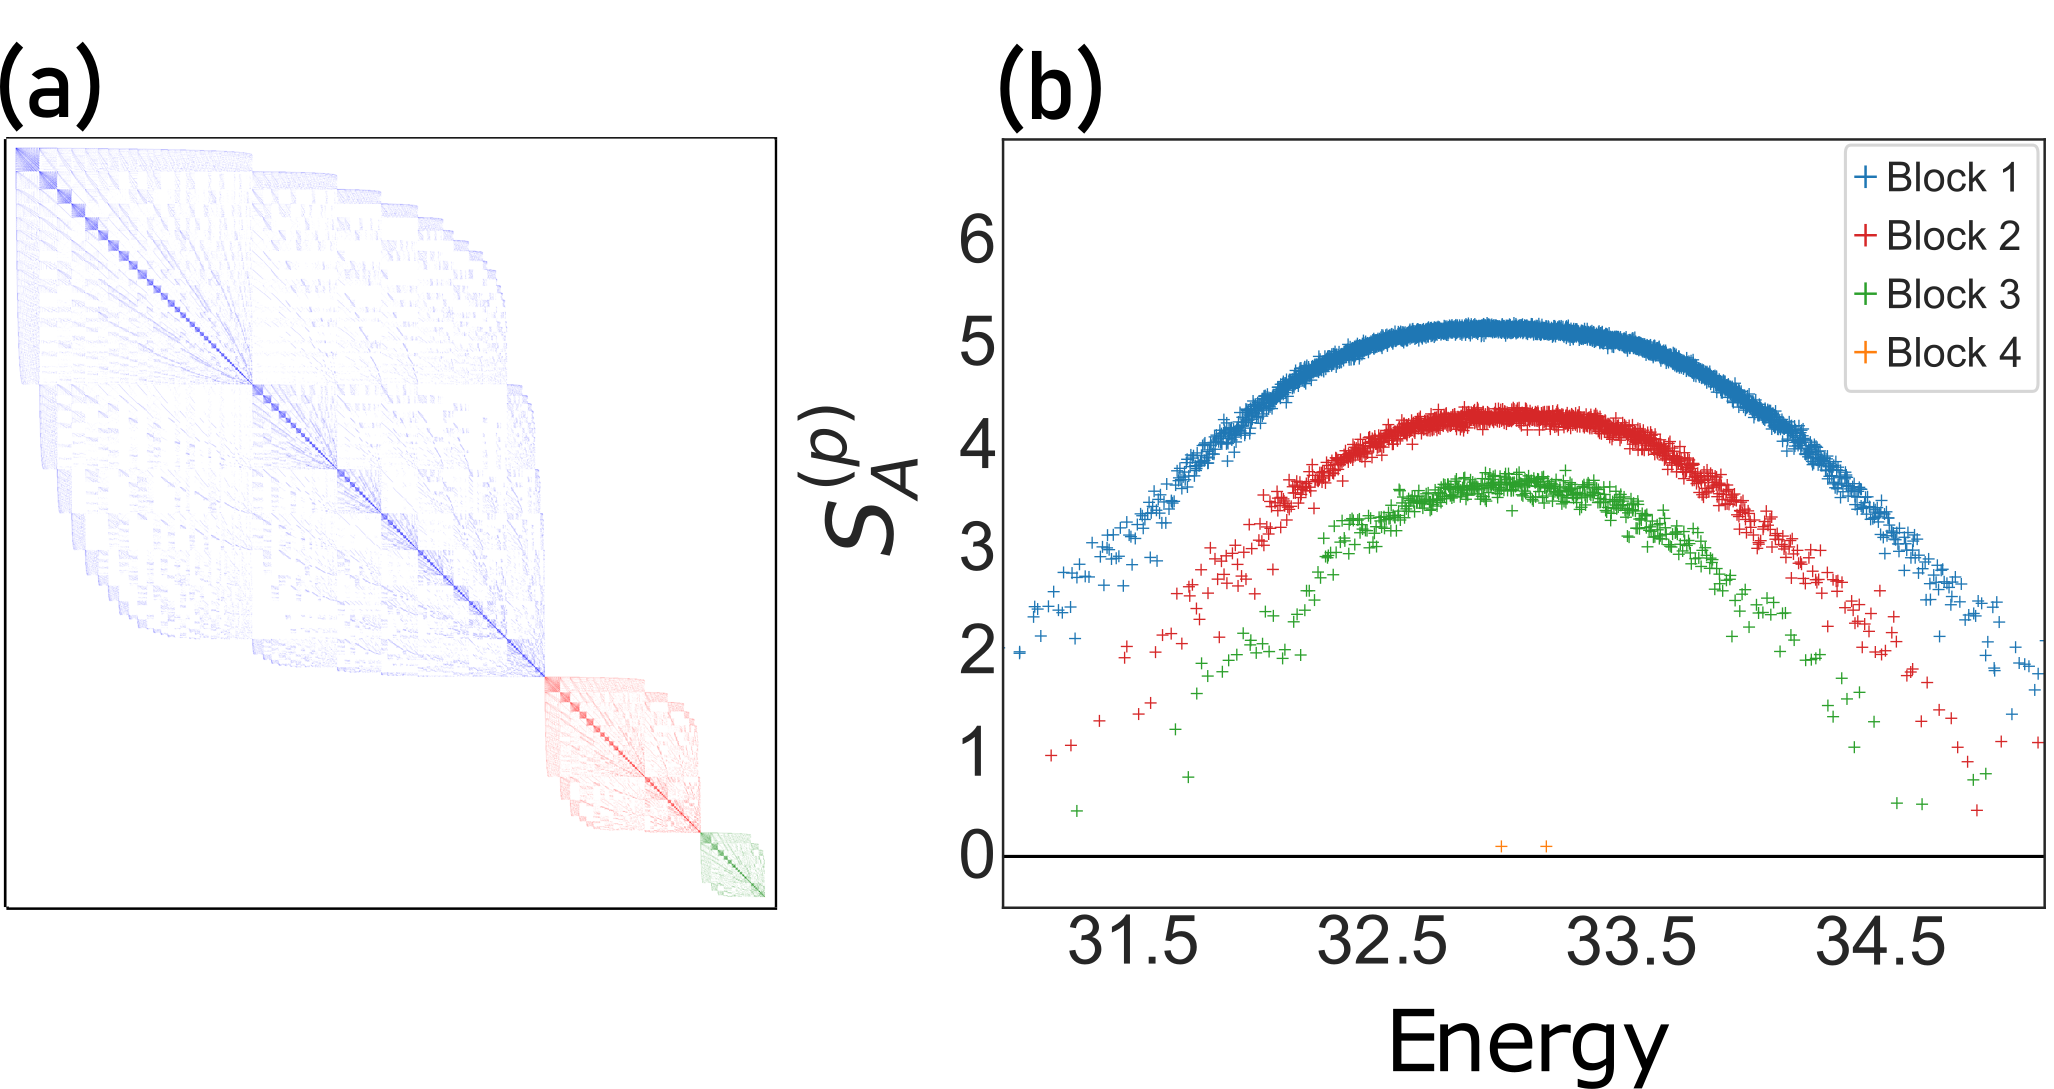
\includegraphics[scale=0.29, width = \linewidth]{figures/block_EEs_p_tot_30_allodds_matrix_side_png-resized.png}
  \caption{(a) Hamiltonian matrix for $\ptot = 30$ with symmetry $T_2$ enforced. White cells are zeroes; blocks are colour-coded. (b) Momentum-space entanglement entropies sorted by energy. Parameter values are as in Fig. \ref{fig:matrices}. We divide the single-particle momentum space [the space $p$ ranges over in Eq.~\eqref{eq:ferm_basis}] into subspaces $A$ and $B$ that correspond to roughly equal Hilbert space dimensions~\cite{Schindler_2022}. Here, for $\ptot = 30$, we choose $A = [-7, 3]$ and $B$ as its complement. These subspaces have Hilbert space dimensions $\mathrm{dim}(\mathcal{H}_A) = 1086$ and $\mathrm{dim}(\mathcal{H}_B) = 996$, while the full Hilbert space has dimension $\mathcal{P}(30) = 5604$ [which is smaller than $\mathrm{dim}(\mathcal{H}_A) \mathrm{dim}(\mathcal{H}_B)$ due to the constraint that the total momentum should be $\ptot$]. Each Hamiltonian block from (a) corresponds to an entropy band in (b).}
\label{fig:onlyEEs}
\end{figure}

\subsection{Numerically observed block distribution}
\label{sec:block_distribs}
We here further study the number of blocks and their relative size against $\ptot$. We measure the amount of fragmentation via the Inverse Participation Ratio (IPR), defined as 
\begin{equation} \label{eq: ipr def}
\text{IPR} = \sum_{i}\frac{d_{i}^2}{D^2}
\end{equation}
where $d_i$ is the dimension of the $i$th block and $D$ is the size of the full Hilbert space at a given $\ptot$. 
There are two characteristic régimes: (1) there is a dominant block and the IPR is almost $1$; (2) there is no dominant block, there are many blocks, and the IPR approaches $0$. To seek the ``most fragmented" pattern then corresponds to minimising the IPR. At a given $\ptot$, the potential configuration that minimises the IPR is the one with the most potentials set equal [Eq.~\eqref{eq:potential_seq}], simply because this destroys the most off-diagonal elements in the corresponding Hamiltonian matrix.

\begin{figure}[t]
  \centering
  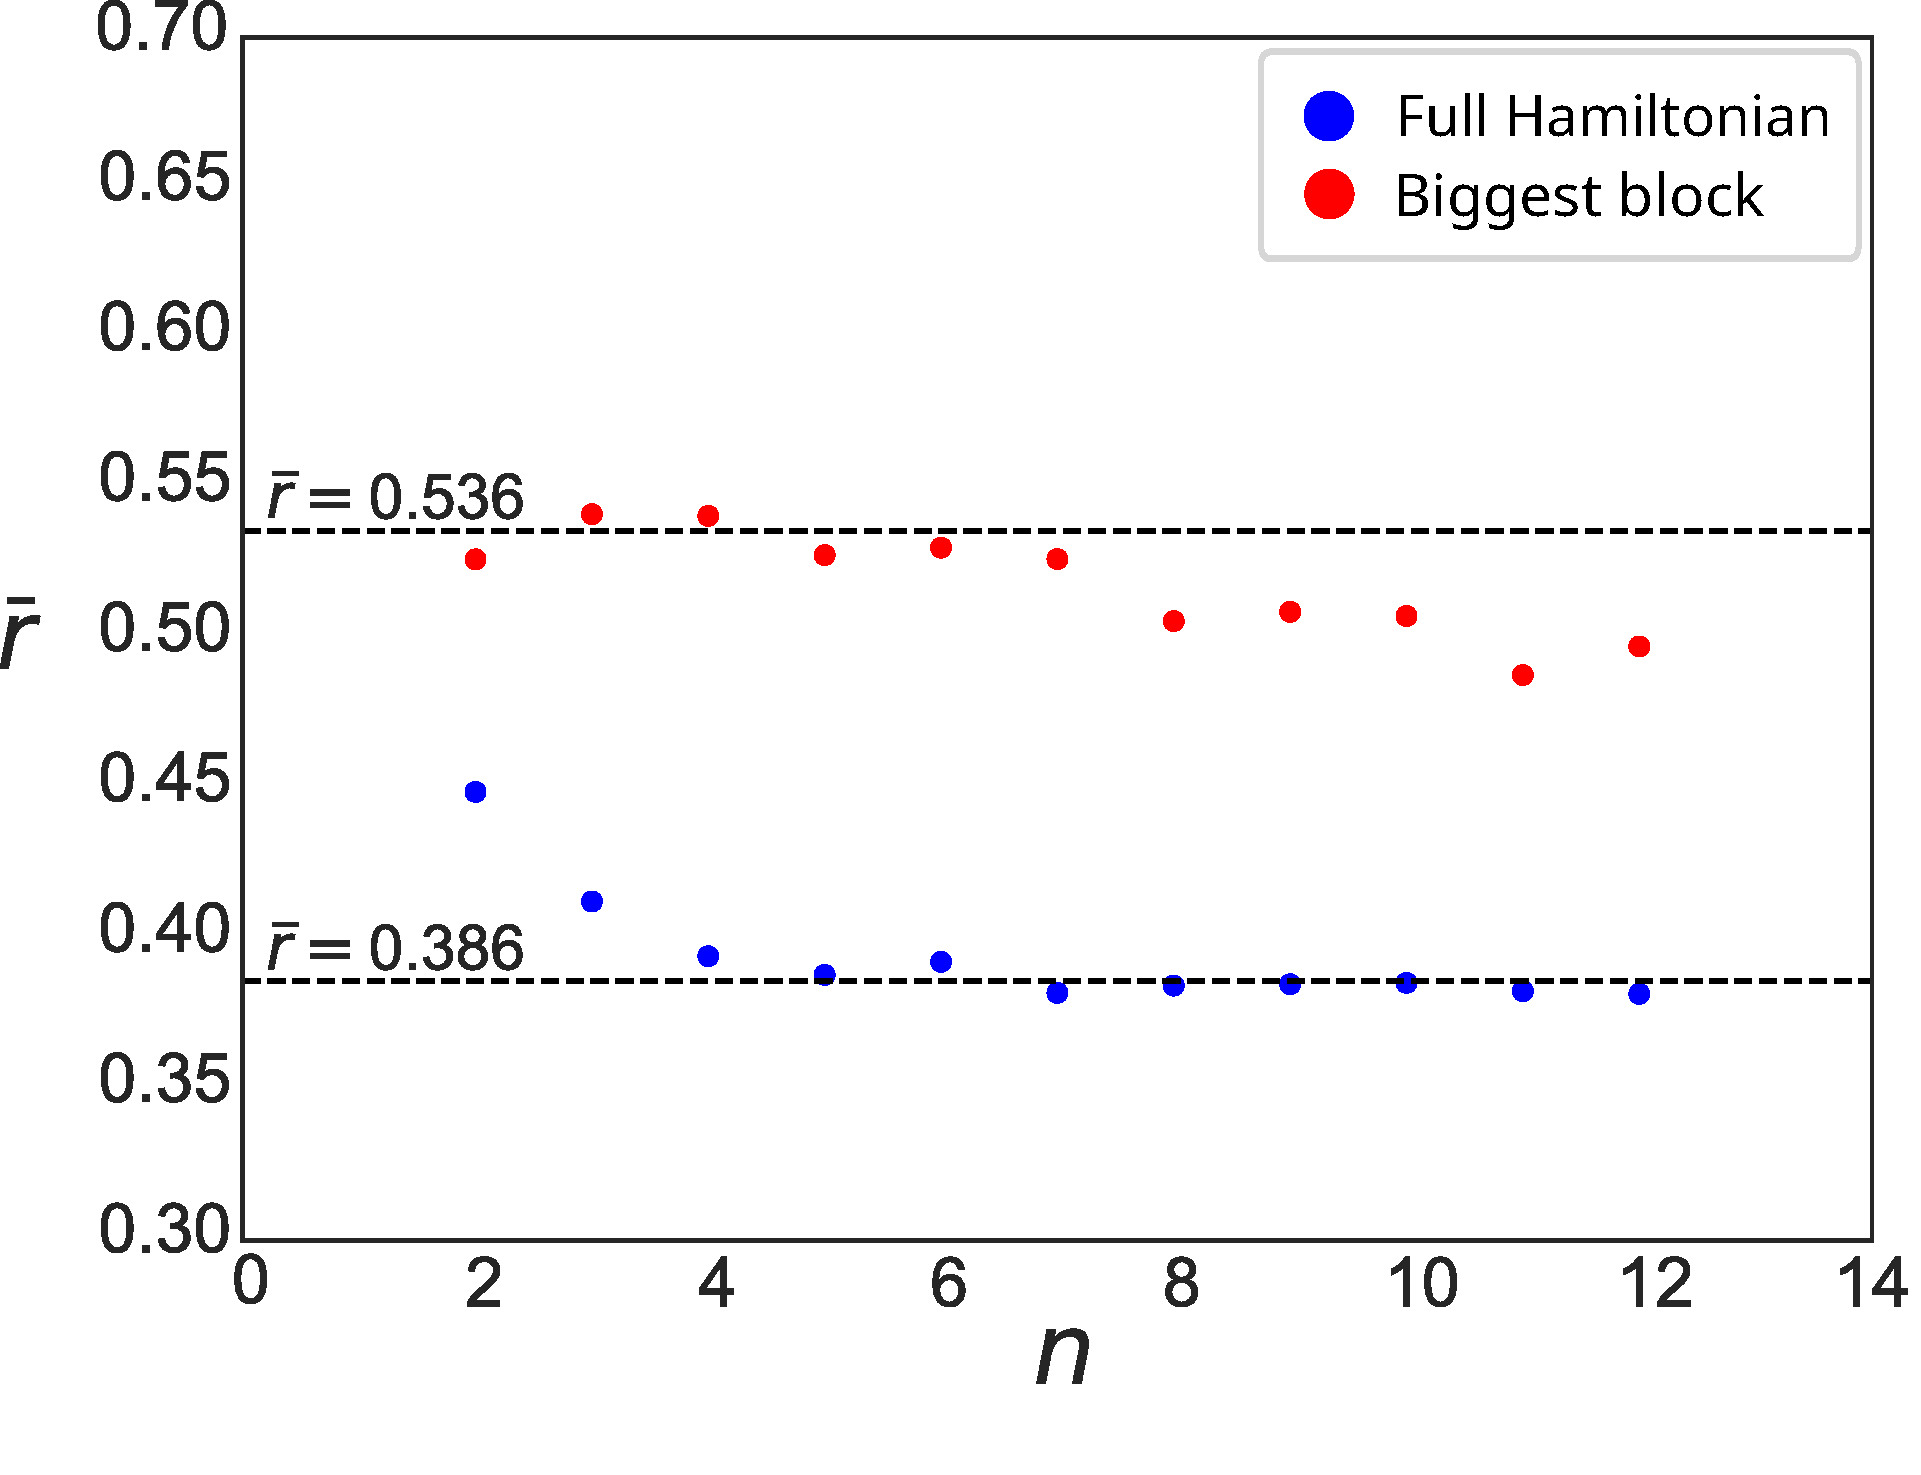
\includegraphics[scale=0.45, width = \columnwidth]{figures/avg_r_against_n_ptot_30_nmin_2_nmax_13_cropped_FINAL.pdf}
  \caption{Average adjacency gap ratio $\bar{r}$ for $\ptot = 30$ when enforcing the various symmetries $T_n$. Numerical parameters are the same as in Fig. \ref{fig:matrices}. Blue points represent the full Hamiltonians' $\bar{r}$, while red points are for the biggest blocks' $\bar{r}$. Dashed horizontal lines represent the (fragmented) Poisson average $\bar{r} \approx 0.386$ and the (thermal) GOE $\bar{r} \approx 0.536$.}
\label{fig:rgraph}
\end{figure}

We compute the IPR for a given symmetry $T_n$ against $\ptot$. The result is shown in Fig. \ref{fig:blockpops}b for $n=2$ (Fig.~\ref{fig:blockpops_n_3}b for $n=3$). We find that, fixing a symmetry $T_n$, the IPR decreases as $\ptot$ increases, indicating that the system becomes increasingly fragmented with $\ptot$.
Moreover, the IPR plots for symmetry $T_n$ decompose into $n$ monotonously decreasing curves corresponding to different values of $p = \ptot \Mod n$, with higher $p$ corresponding to lower IPR. This behaviour can be qualitatively understood by computing the fraction $f$ of potentials $V(p)$ set equal [Eq.~\eqref{eq:potential_seq}] to enforce a given symmetry $T_n$. $f$ is a measure of how constrained the dynamics are, and should therefore correlate with the number of blocks. For $\ptot = kn + p, \; k \in \mathbb{Z}, \; p \in [1, n - 1]$, we have $f = \frac{k(n-1) + p}{kn}$, which increases with $p$. Thus we expect higher $p$ to be more fragmented.

Additionally, we can use the sequence $a_2(j)$ to obtain an upper bound for the scaling of the IPR for $n=2$. Using the asymptotic scaling given on the sequence's OEIS page~\cite{OEIS_sequence},
\begin{equation}
    a_2(j) \sim \frac{e^{2\pi\sqrt{j/3}}}{4 \cdot 3^{3/4}\cdot j^{5/4}}\left[1 + \mathcal{O}\left(\frac{1}{j^{1/2}}\right)\right],
\end{equation}
it follows that the IPR for $n=2$ is bounded from above:
\begin{equation}
    \text{IPR}_2(\ptot) \leq \frac{2^{5/4}3^{1/2}}{\ptot^{1/2}} + \mathcal{O}\left(\frac{1}{\ptot^{7/4}}\right),
\end{equation} 
and tends to zero as $\sim 1/\sqrt{\ptot}$ when $\ptot \rightarrow \infty$. 
Thus, we obtain a \textit{strongly} fragmented system~\cite{Moudgalya_2022} in the thermodynamic limit in which $L$ is sent to infinity but the physical momentum (and kinetic energy scale) are held fixed.

For any $n$ non-prime, let $\{f_{1}, f_{2}, f_{3}...\}$ be its factors sorted in increasing order. The $T_n$ block pattern can be regarded as first resolving only $T_{f_1}$, then the corresponding blocks `split' into smaller blocks when further resolving $T_{f_2}$, and so on. Suppose each $T_{f_1}$ block of size $d_i$ splits into $T_{f_2}$-resolved blocks $d_{j_i}$ such that $\sum_j d_{j_i} = d_i$. Then the $T_{f_2}$-and-$T_{f_1}$-resolved IPR will be $\sum_j \sum_i d_{j_i}^2/D^2$. But by the triangle inequality, $\sum_j d_{j_i}^2 \leq {(\sum_j d_{j_i})}^2 = d_i^2$, so this IPR will necessarily be smaller than the $T_{f_1}$-only-resolved IPR. Thus, the IPR for $n$ non-prime is necessarily smaller than the IPR of any of its factors. Using the above result for $n=2$, this implies that the block distribution resulting from $T_n$ with any even $n$ will also have an IPR decaying at least as $1/\sqrt{\ptot}$ when $\ptot \rightarrow \infty$.

\section{Thermalisation in fragmented blocks: The case of $T_2$} \label{sec:entropyandlvlstats}

We now analyse the thermal properties of the fragmented blocks that result from the symmetry $T_2$.
Using the method outlined in Ref.~\onlinecite{Schindler_2022}, we compute the distribution of momentum-space entanglement entropies for eigenstates of a generic realisation of the CNLLL Hamiltonian that commutes with $T_2$. Fig. \ref{fig:onlyEEs}b shows the entanglement entropies for $\ptot = 30$. Here, each block in the Hamiltonian corresponds to a distinct entropy band. The rough magnitude of entropies in each band scales with the size of the corresponding block. 

We also study the adjacency gap ratio statistics, which improves upon simple energy level statistics~\cite{LevelSpacingStats}.
Since ${H}$ is purely real, the Wigner-Dyson distribution of interest is the Gaussian orthogonal ensemble (GOE), with an average of gap ratio $\bar{r} \approx 0.536$, indicating thermalisation. 
In comparison, the Poisson distribution displayed by strongly fragmented systems has average $\bar{r} \approx 0.386$. We show the detailed distributions for the symmetry $T_2$ and $\ptot = 30$ in Appendix \ref{appendix:LevelStats}. As shown in the overview Fig.~\ref{fig:rgraph}, although each separate block follows GOE statistics, the full Hamiltonian has statistics between Poisson and GOE, with a mean $\bar{r} \approx 0.444$. It is thus fragmented, albeit not `fully' Poisson. As discussed in section \ref{sec:symmetries}, symmetries $T_n$ with larger $n$ are more fragmented and the full Hamiltonian level statistics become increasingly Poisson while each individual block remains thermal. This is illustrated in Fig. \ref{fig:rgraph}, where we plot the level statistics' $\bar{r}$ value for each symmetry $T_n$ for $\ptot=30$.

There is one caveat: as $n$ increases and $\ptot$ is held fixed, the largest block's relative size decreases, implying that the quality of the GOE fit decreases. This explains why the red dots do not converge well in $\bar{r}$. This is a finite-size effect: plotting the same symmetry $T_n$'s level statistics for increasing $\ptot$ gives a $\bar{r}$ value that always approaches the GOE value.

\section{Summary \& Outlook}
\label{sec:conclusion}
We have found an infinite family of unconventional symmetries $T_n$ that yield HSF in the CNLLL. They provide a spectrum of various degrees of strong fragmentation between $n=2$ and $n \to \infty$ (for $\ptot \to \infty$). The corresponding Hamiltonians become strongly fragmented in the limit of large total momenta (large Hilbert space sizes). For a fixed instance of the interaction potential $V(p)$, each Hamiltonian block's level statistics are individually of the Wigner-Dyson type, indicating that eigenstates within each block thermalise with each other.

We now list a few open questions. The first is whether there exist other interesting patterns of fragmentation in the CNLLL. We performed an exhaustive search (up to $\ptot \leq 10$) for HSF beyond the mechanism described here, which consists of setting equal all interaction potentials $V(p)$ in the set $P_n$ [(Eq.~\eqref{eq:potential_seq})]. Within this range of $\ptot$, we only found HSF for $V(p)$ potential tuning patterns that are directly inherited from $P_n$ by removing some of the higher-momentum $V(p)$'s.

We must also stress here that we searched for fragmentation \textit{only} in the fermionic basis - this amounts to determining whether a given choice of interaction potentials $V(p)$ allows the fermionic-basis Hamiltonian matrix to be permuted into block-diagonal form. The existence of further families producing HSF is possible as well and warrants further investigation.

Also, Ref.~\onlinecite{PhysRevX.12.011050} characterises HSF in terms of \textit{commutant algebras}; these are algebras of operators commuting with every term in the Hamiltonian. It could be instructive to explicitly find the commutant algebra for the $V(p)$ potential tuning pattern $P_n$ studied here, which may actually be larger than the algebra of symmetries $T_n$.

\acknowledgments{AC and NR thank Kevin Buzzard for discussions regarding the sequence $a_2(j)$. FS thanks Sanjay Moudgalya for help in clarifying the notion of Hilbert space fragmentation. FS also thanks Nicolas Regnault and Andrei Bernevig for an earlier collaboration on a similar topic. AC acknowledges funding from the Imperial College London President's PhD Scholarships. HD acknowledges support from the Engineering and Physical Sciences Research Council (grant number EP/W524323/1). FS gratefully acknowledges support from the Simons Center for Geometry and Physics, Stony Brook University at which some of the work for this paper was performed.}

\bibliography{refs}

\appendix

\begin{figure*}[t]
  \centering
  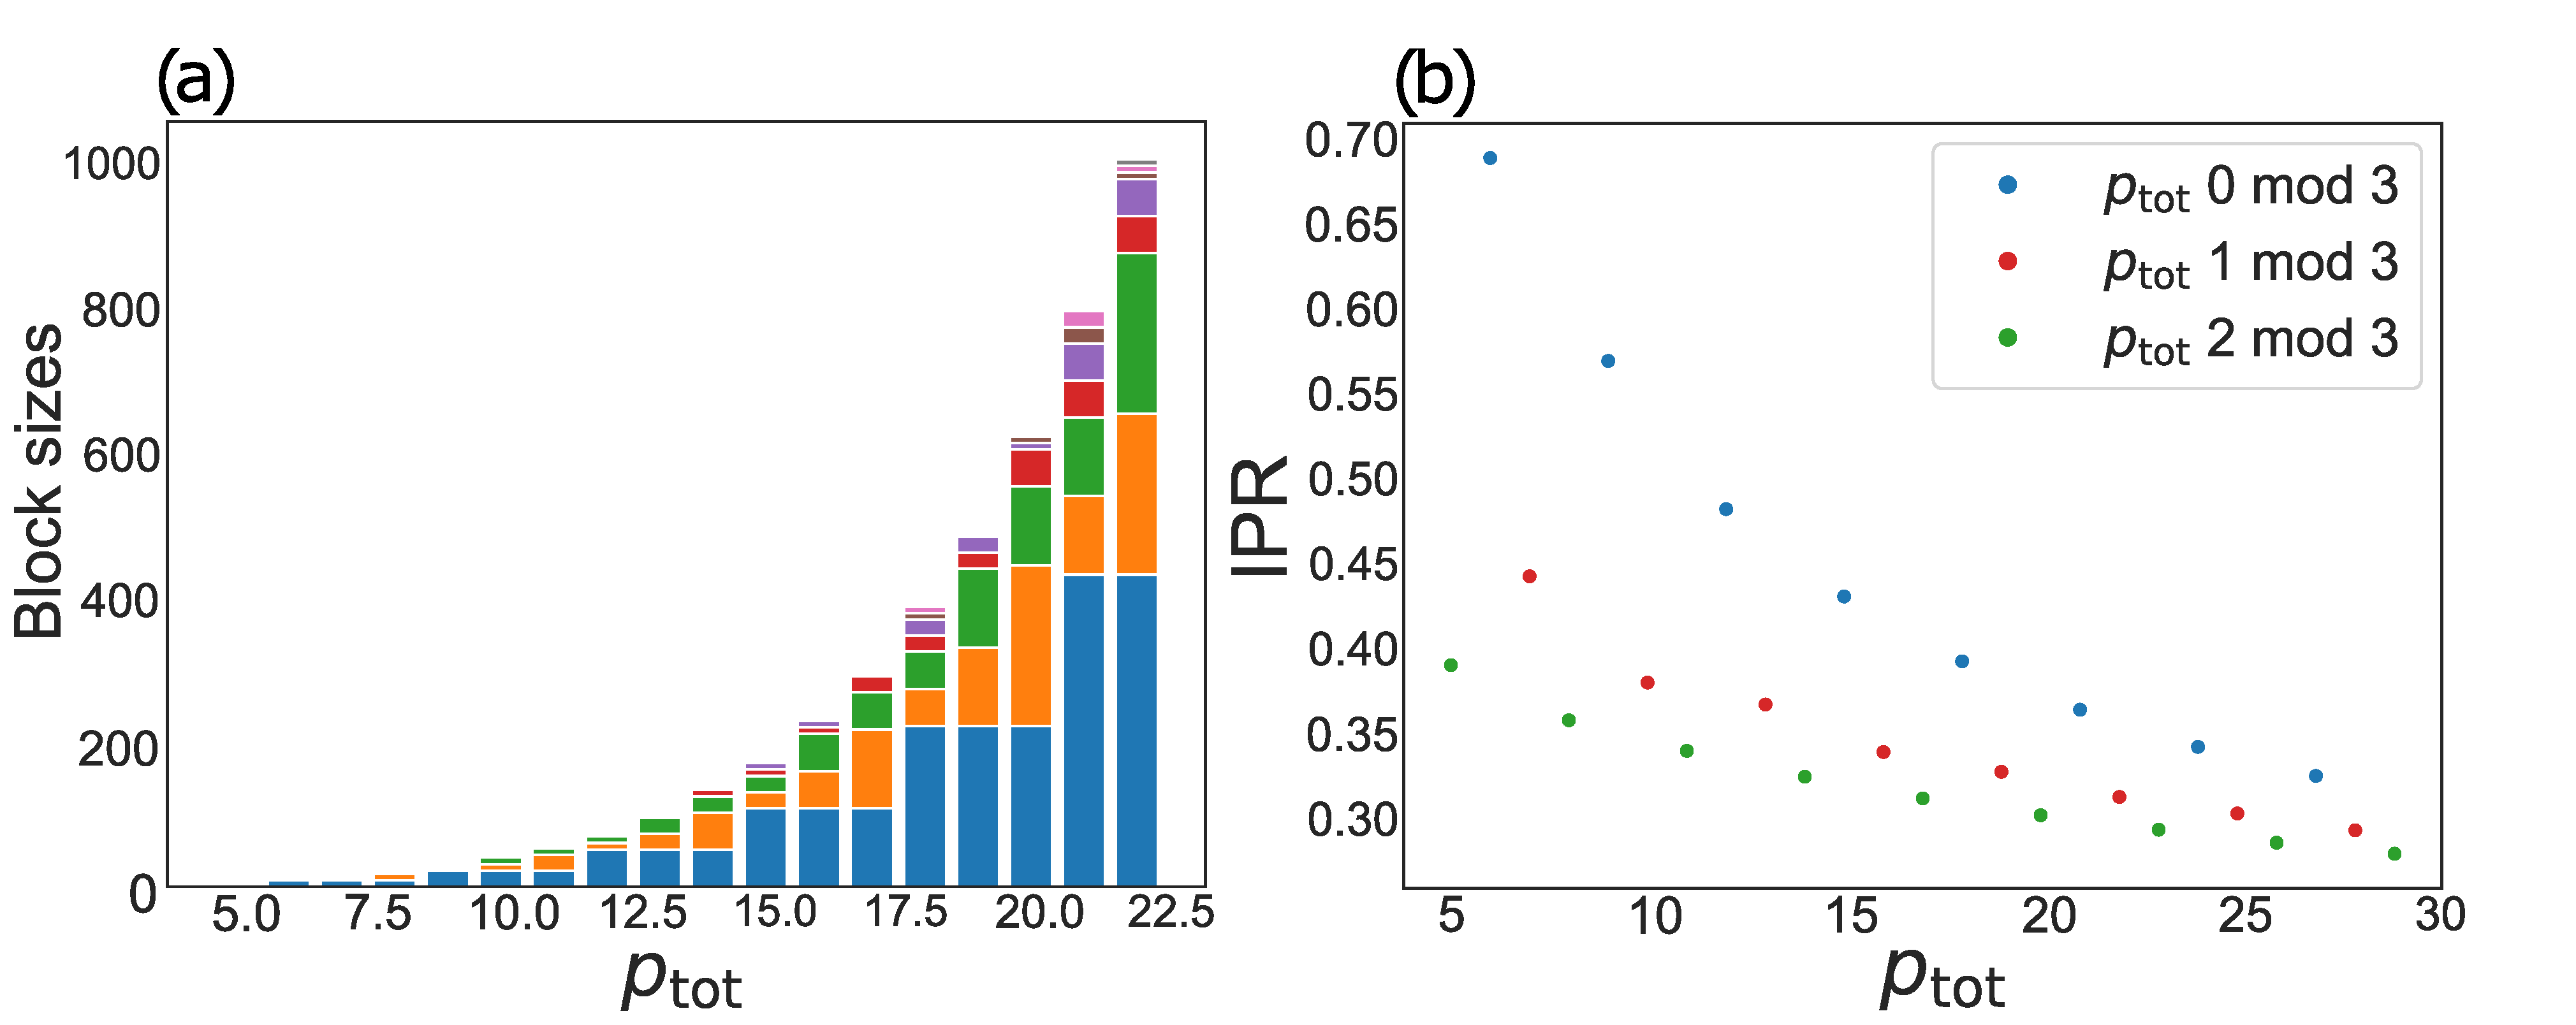
\includegraphics[width = 0.8\linewidth]{figures/blocks_and_iprs_n_3_BIGGER.pdf}
  \caption{Same as Fig. \ref{fig:blockpops} but for symmetry $T_3$. (a) Stacked-bar histograms of block sizes. At a given $\ptot$ there are more blocks for symmetry $T_3$ than $T_2$. (b) IPR against $\ptot$. The IPR still tends to 0 for all patterns in the family. We colour-code the $\ptot$ off different moduli with respect to $n=3$.}
\label{fig:blockpops_n_3}
\end{figure*}

\section{Momentum-Space Commutator}
\label{appendix:derivation}
Here we show that the operator $T_n$ becomes a symmetry of the Hamiltonian under pattern $P_n$. Recall that
\begin{equation}
T_n = \sum_{p}e^{ip\theta_n} c^{\dag}_{p}c_p,
\end{equation}
where $\theta_n = 2\pi/n$. The sum goes over all $p \in \mathbb{Z}$, but could be restricted to the range $\left[-p_{\mathrm{tot}}+1, p_{\mathrm{tot}}\right]$ within a given $p_{\mathrm{tot}}$ sector, since roughly speaking, summing all nth roots of unity gives zero. 
To see that $T_n$ is a symmetry, we compute the commutator of $T_n$ with ${H_{\mathrm{int}}}$ as in Eq.~\eqref{eq:hint} as follows. Consider
\begin{equation}
c_l^{\dag} c_l c_{q+p}^{\dag} c_q c_k c_{k-p}^{\dag}.
\end{equation}
We use the anti-commutation relations to move $n_l = c_l^{\dag} c_l$ to the right end of this string. Doing so and rearranging yields
\begin{flalign}
& \left[c_l^{\dag} c_l, c_{q+p}^{\dag} c_q c_k c_{k-p}^{\dag}\right] = \notag \\ & \delta_{l, q+p}c_l^{\dag} c_{q}c_{k}c_{k-p}^{\dag} +  \delta_{l, k-p}c_{q+p}^{\dag} c_{q}c_{k}c_{l}^{\dag} \notag \\ & - \delta_{lq}c_{q+p}^{\dag} c_{l}c_{k}c_{k-p}^{\dag} - \delta_{lk}c_{q+p}^{\dag} c_{q}c_{l}c_{k-p}^{\dag}.
\end{flalign}
Multiplying by $e^{i\theta_n l}$ and summing over the index $l$, we get
\begin{flalign}
 & \left[T_n, c_{q+p}^{\dag} c_q c_k c_{k-p}^{\dag}\right] = \notag \\  & c_{q+p}^{\dag} c_{q}c_{k}c_{k-p}^{\dag} \left[e^{i\theta_n (q+p)} + e^{i\theta_n (k-p)} - e^{i\theta_n q} - e^{i\theta_n k} \right].
\end{flalign}
Thus when summing over $q, k$, we have
\begin{flalign}
& \left[T_n, \ {H_{\mathrm{int}}}\right] = \notag  \\ & \sum_{q>k}\sum_{p > (k-q)/2} \left[V(q-k+p) - \delta_{p \neq 0}V(p) \right] \times \notag \\ & \hspace{4cm} \left[T_n, c_{q+p}^{\dag} c_q c_k c_{k-p}^{\dag}\right] \notag \\ & = \sum_{q > k}\sum_{p > (k-q)/2} \left[V(q-k+p) - \delta_{p \neq 0}V(p) \right] F_n(q,k,p),
\end{flalign}
where we have defined
\begin{equation}
    F_n(q,k,p) = e^{i\theta_n (q+p)} + e^{i\theta_n (k-p)} - e^{i\theta_n q} - e^{i\theta_n k},
\end{equation}
and note that $F_n$ vanishes precisely when at least one of $p, q-k+p$ is a multiple of $n$. When $p$ is a multiple of $n$ the first and third term cancel each other, as do the second and fourth; when $q-k+p$ is a multiple of $n$ the first cancels the fourth and the second cancels the third. 
Hence for the commutator to vanish completely, the other square bracket term, $V(q-k+p) - \delta_{p \neq 0}V(p)$, must vanish when $p$ and $q-k+p$ are both \textit{not} multiples of $n$. Thus $T_n$ is a symmetry when all $V(p)$ are set equal for all $p$ not multiples of $n$, i.e. when we use pattern $P_n$.

\section{Real-space interpretation}
Using the Fourier Transform of $c_p$ and $\cdag_p$ operators, we write 
\begin{equation}
  \begin{aligned}
T_n &= \frac{1}{L}\sum_{p}\int_{x=-L/2}^{L/2} \mathrm{d} x \, c^{\dag}_{x}e^{ipx}\int_{y=-L/2}^{L/2} \mathrm{d} y \, c_ye^{-ipy} e^{ip\theta_n} \\
&= \frac{1}{L}\int_{x=-L/2}^{L/2} \mathrm{d} x \, \int_{y=-L/2}^{L/2} \mathrm{d} y \, c^{\dag}_{x}c_y \sum_{p} e^{ip(x-y+\theta_n)}.
  \end{aligned}
\end{equation}
Using the Dirac comb relation $\sum_{p \in \mathbb{Z}} e^{ipz} = 2\pi\sum_p \delta(z - 2p\pi)$ and $L = 2\pi$, we get
\begin{equation}
  \begin{aligned}
T_n& =\\& \frac{2\pi}{L}\int_{x=-\pi}^{\pi} \mathrm{d} x \int_{y=-\pi}^{\pi} \mathrm{d} y \, c^{\dag}_{x}c_y \sum_{p} \delta(x-y+\theta_n - 2p\pi) \\
&= \sum_{q}\int_{-\pi}^{\pi} \mathrm{d} x \, c^{\dag}_{x}c_{x-\theta_n+2q\pi},
  \end{aligned}
\end{equation}
where now the sum over $q$ is only for $q$ such that $x-y+\theta_n - 2q\pi = 0$ is possible. One can show that this is only possible for $q=0$ and $q=1$. Thus the real-space operators are
\begin{equation}
T_n = \int_{-\pi}^{\pi} \mathrm{d} x \, \cdag_x \left[c_{x-\theta_n} + c_{x + 2\pi - \theta_n}\right].
\end{equation} 
For a one-body state, each term in this expression can be interpreted as rotating the fermion's position from one place on the circle to another; for a many-body state, every fermion is moved in this way.

\section{Real-space commutator}
Consider now the real-space commutator, i.e. the commutator of the real space expressions for $T_n$ and ${\Hint}$. In a similar manner, consider
\begin{equation}
\left[c_x^{\dag} c_{x+\theta_n}, c_{q+p}^{\dag} c_q c_k c_{k-p}^{\dag}\right],
\end{equation}
which by using real-space anti-commutation relations yields
\begin{flalign}
& \delta(x + \theta_n - y)\cdag_xc_y\cdag_zc_z - \delta(x+\theta_n - z)\cdag_x\cdag_yc_yc_z \notag \\ & + \delta(x-y)\cdag_y\cdag_zc_zc_{x+\theta_n} - \delta(x-z)\cdag_yc_y\cdag_zc_{x+\theta_n}.
\end{flalign}
Computing $\left[T_n, \cdag_yc_y\cdag_zc_z\right]$ amounts to integrating this over $x$. Rearranging two of the terms so all indices are of the form $r \pm {\theta_n}$ within the first two operators yields
\begin{equation}
\begin{gathered}
\cdag_{y-\theta_n}c_y\cdag_zc_z + \cdag_{z-\theta_n}c_z\cdag_yc_y - \cdag_yc_{y+\theta_n}\cdag_zc_z - \cdag_zc_{z+\theta_n}\cdag_yc_y \\
+ \delta(z-y-\theta_n)\cdag_yc_z + \delta(y-z-\theta_n)\cdag_zc_y \\ - \delta(y-z)\cdag_{z+\theta_n}c_y - \delta(y-z)\cdag_yc_{z+\theta_n}.
\end{gathered}
\end{equation}
Now multiplying by $\frac{1}{2}V(y-z)$ and integrating over two copies of $S^1$ in $y, z$ yields the full commutator $\left[T_n, {\Hint}\right]$ as
\begin{equation}
\begin{aligned}
&\frac{1}{2}\int \mathrm{d} y \mathrm{d} z \, V(y-z)\left[\cdag_{y-\theta_n}c_y\cdag_zc_z - \cdag_yc_{y+\theta_n}\cdag_zc_z\right] \notag \\ & + \frac{1}{2}\left[V(\theta_n) - V(0) \right] \int \mathrm{d} y \, \left[\cdag_yc_{y+\theta_n} + \cdag_{y-{\theta_n}}c_y\right].
\end{aligned}
\end{equation}
Now changing variables to $y' = y + \theta_n$ for the second term of the first integral and the second term of the second integral, using periodic boundary conditions and relabelling $y' \rightarrow y$ gives
\begin{flalign}
\frac{1}{2}\int \mathrm{d} y \mathrm{d} z \,& \left[V(y-z) -V(y-z-\theta_n) \right]\cdag_{y-\theta_n}c_y\cdag_zc_z \notag \\ & + \frac{1}{2}\left[V(\theta_n) - V(0) \right] \int \mathrm{d} y \, \cdag_{y-\theta_n}c_y.
\end{flalign}
For this commutator to vanish, we seem to need $V(x+\theta_n) = V(x) \; \forall x \in S^1$. In particular it suggests $V(0) = V(\theta_n)$, which when Fourier transforming implies 
\begin{equation}
\sum_{\text{p not multiple of n}} V(p)\left(e^{i\theta_n p} - 1\right) = 0,
\end{equation}
which e.g. for $n=3$ gives
\begin{flalign}
&V(1)\left(e^{i2\pi/3}-1\right) +  V(2)\left(e^{i4\pi/3}-1\right) +\notag \\  &V(4)\left(e^{i2\pi/3}-1\right) + V(5)\left(e^{i4\pi/3}-1\right) + \ldots = 0,
\end{flalign}
which is only true if both $V(1) + V(4) + \ldots = 0$ and $V(2) + V(5) + \ldots = 0$. If we use pattern $P_3$, we then minimally require $V(1) = V(2) = 0$. For general $n$, we require $V(1)=V(2)=\ldots=V(n-1) = 0$. This agrees with the momentum-space commutator, with the extra requirement that every term in $P_n$ be set to $0$. We believe this results from the absence of normal-ordering of the Hamiltonian in the real-space derivation. 

\begin{figure}[t]
  \centering
  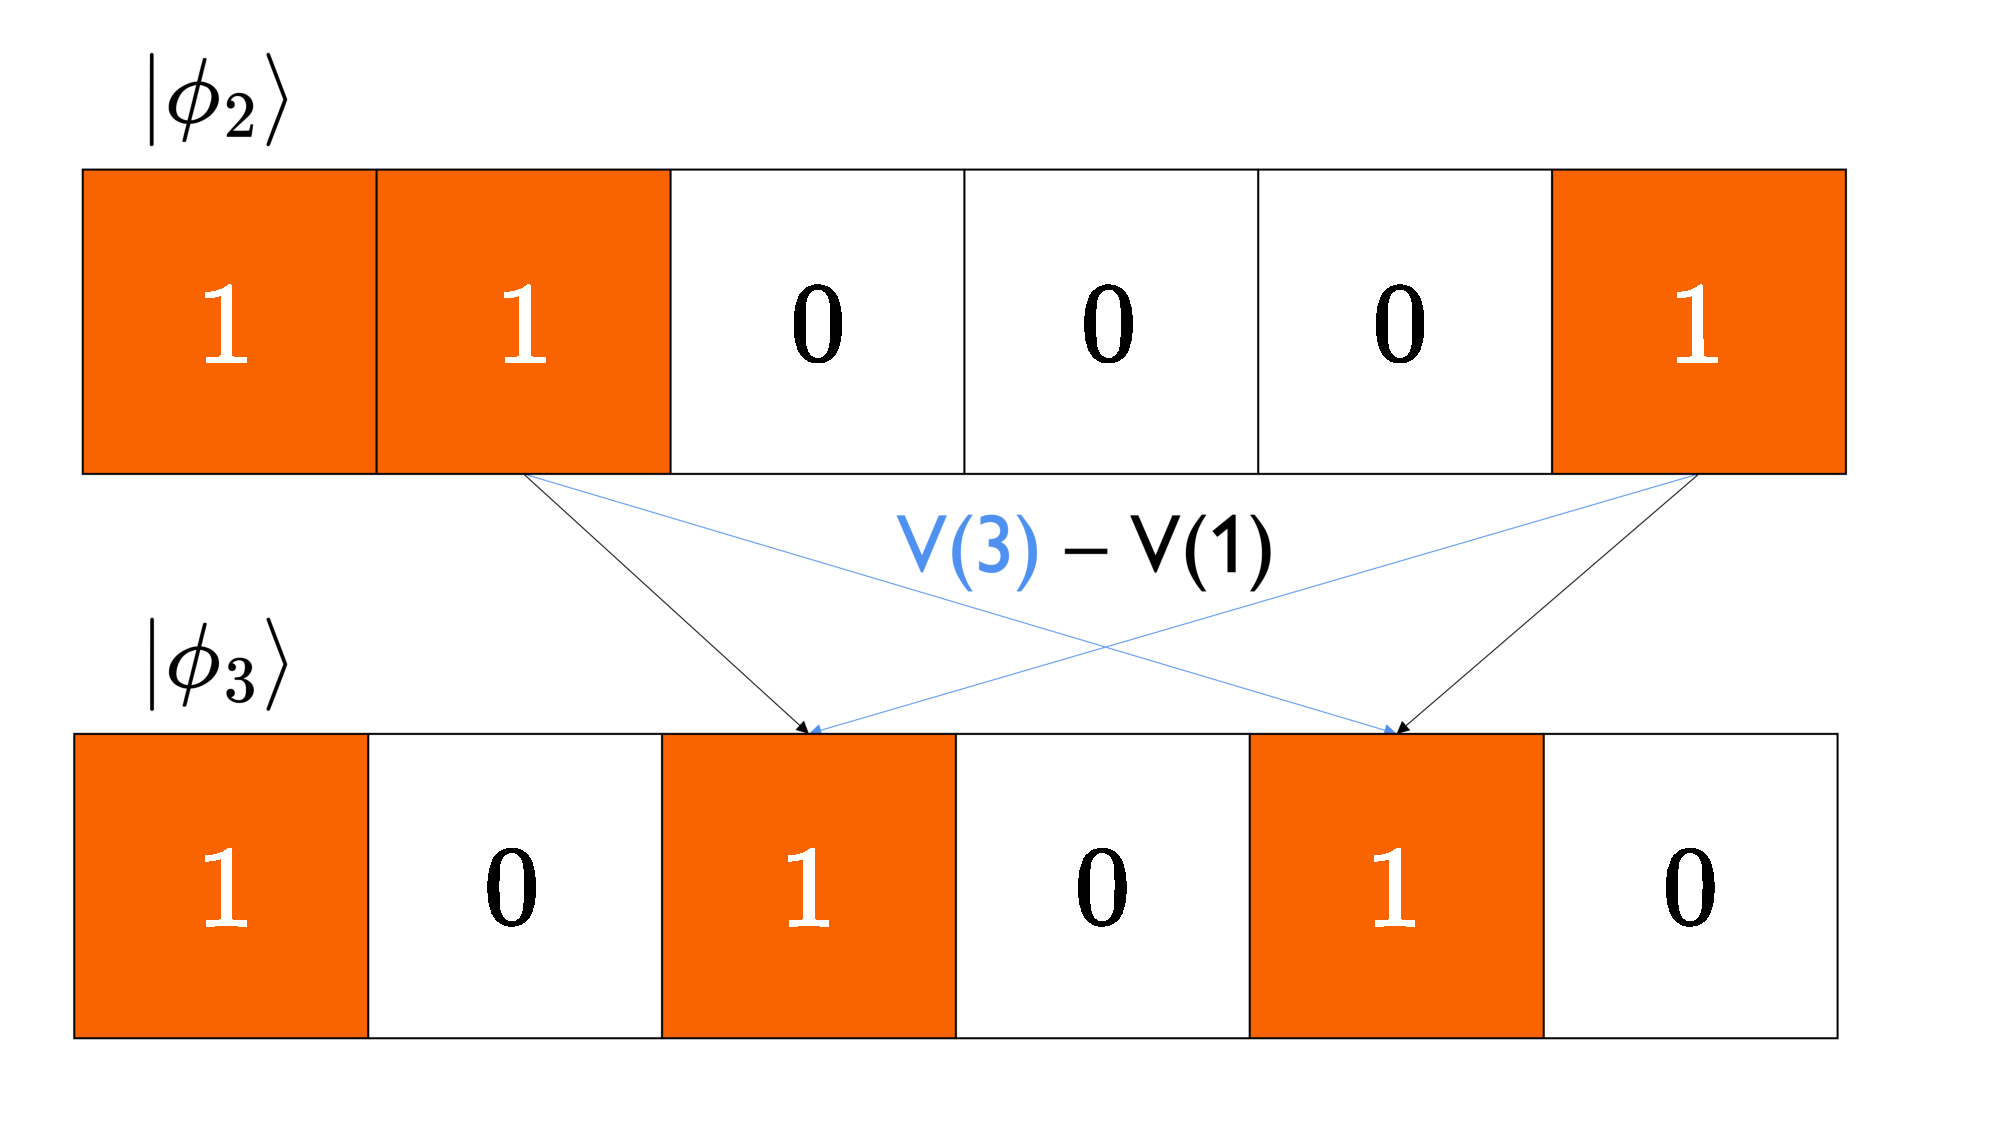
\includegraphics[scale = 0.2]{figures/binary_scatter.pdf}
  \caption{Example of a scatter computation between two states. States are represented by binary strings indicating which momenta are occupied (1s) and which are not (0s). Scattering between two states uses the XOR operation between these two binaries, and finds the two possible permutations to get the scattering term, here $V(3) - V(1)$.}
\label{fig:examplescatter}
\end{figure}

\begin{figure}[t]
    \centering
    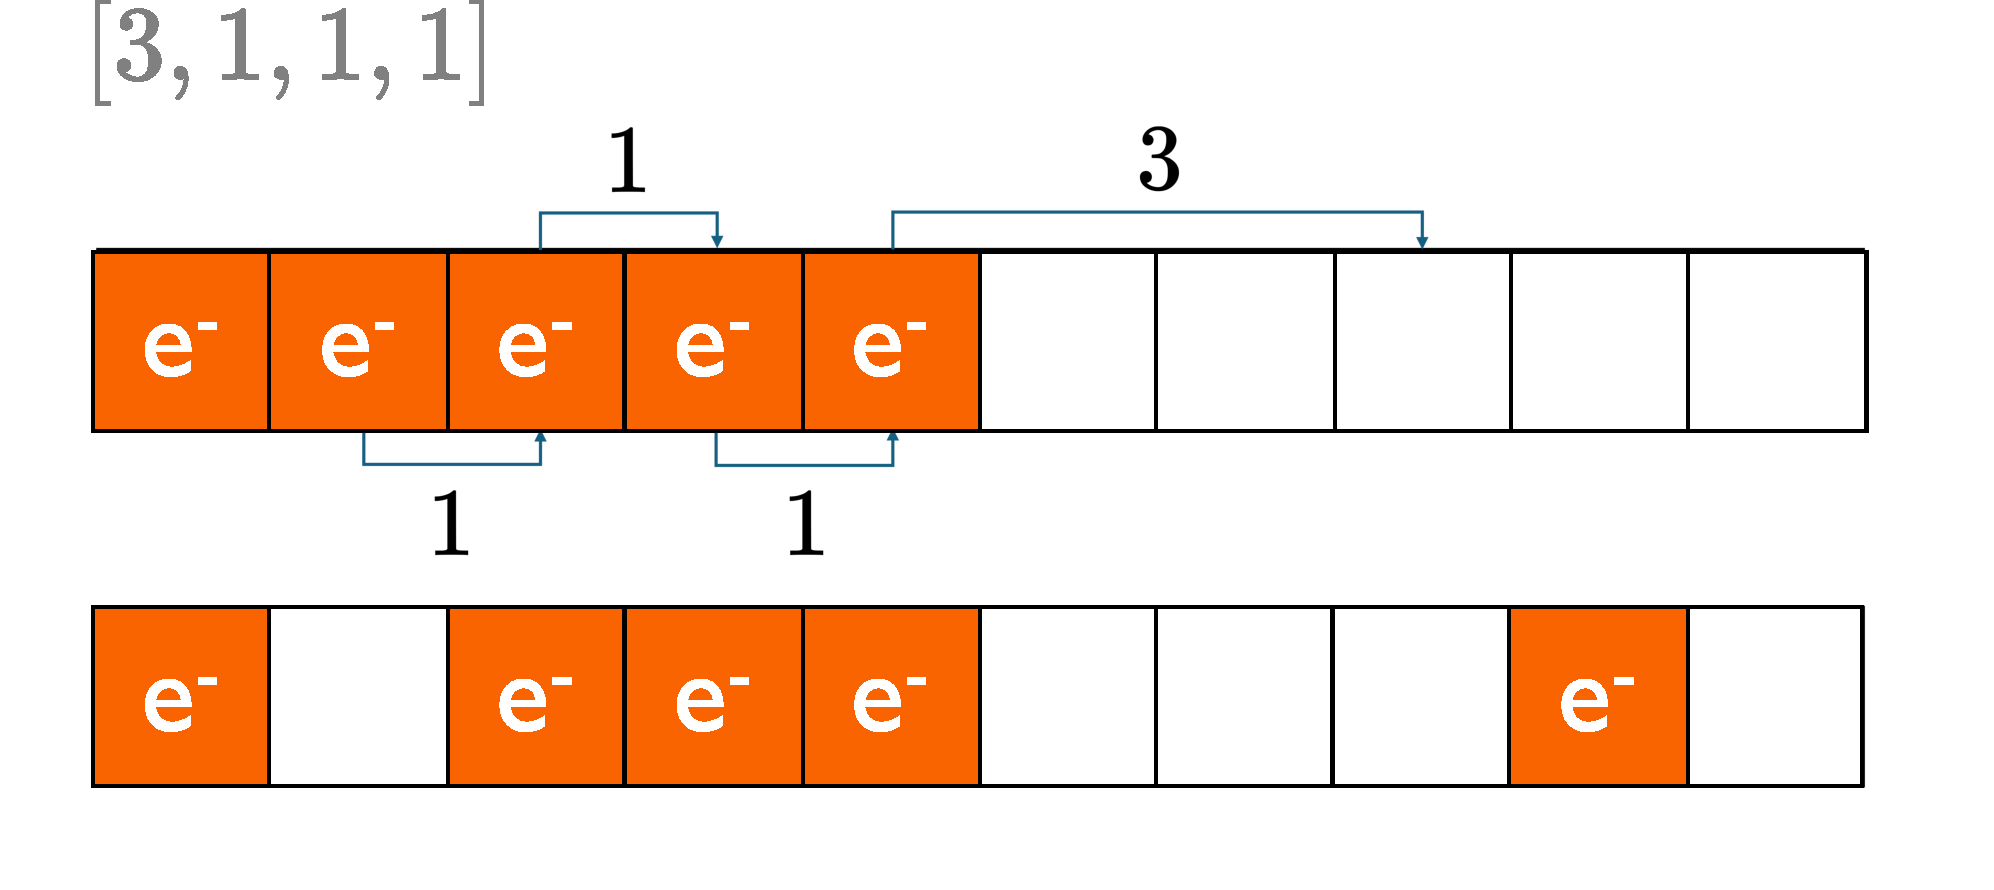
\includegraphics[scale = 0.45, width = \columnwidth]{figures/partition_parity_example.pdf}
    \caption{Representation of how states with the same $n_{\text{e}}-n_{\text{o}}$ numbers can be generated from one another via partitions in the set $S_{oe}$. Here, $c_3^{\dagger}c_{-3}\ket{\Omega}$ (second row) is created from $\ket{\Omega}$ (first row) via the partition $[3, 1, 1, 1]$ in $S_{\text{oe}}(6)$. Both have $n_{\text{e}}-n_{\text{o}} = 0$ because the partition is in $S_{\text{oe}}$.}
    \label{fig:boring}
\end{figure}

\begin{figure*}[t]
  \centering
  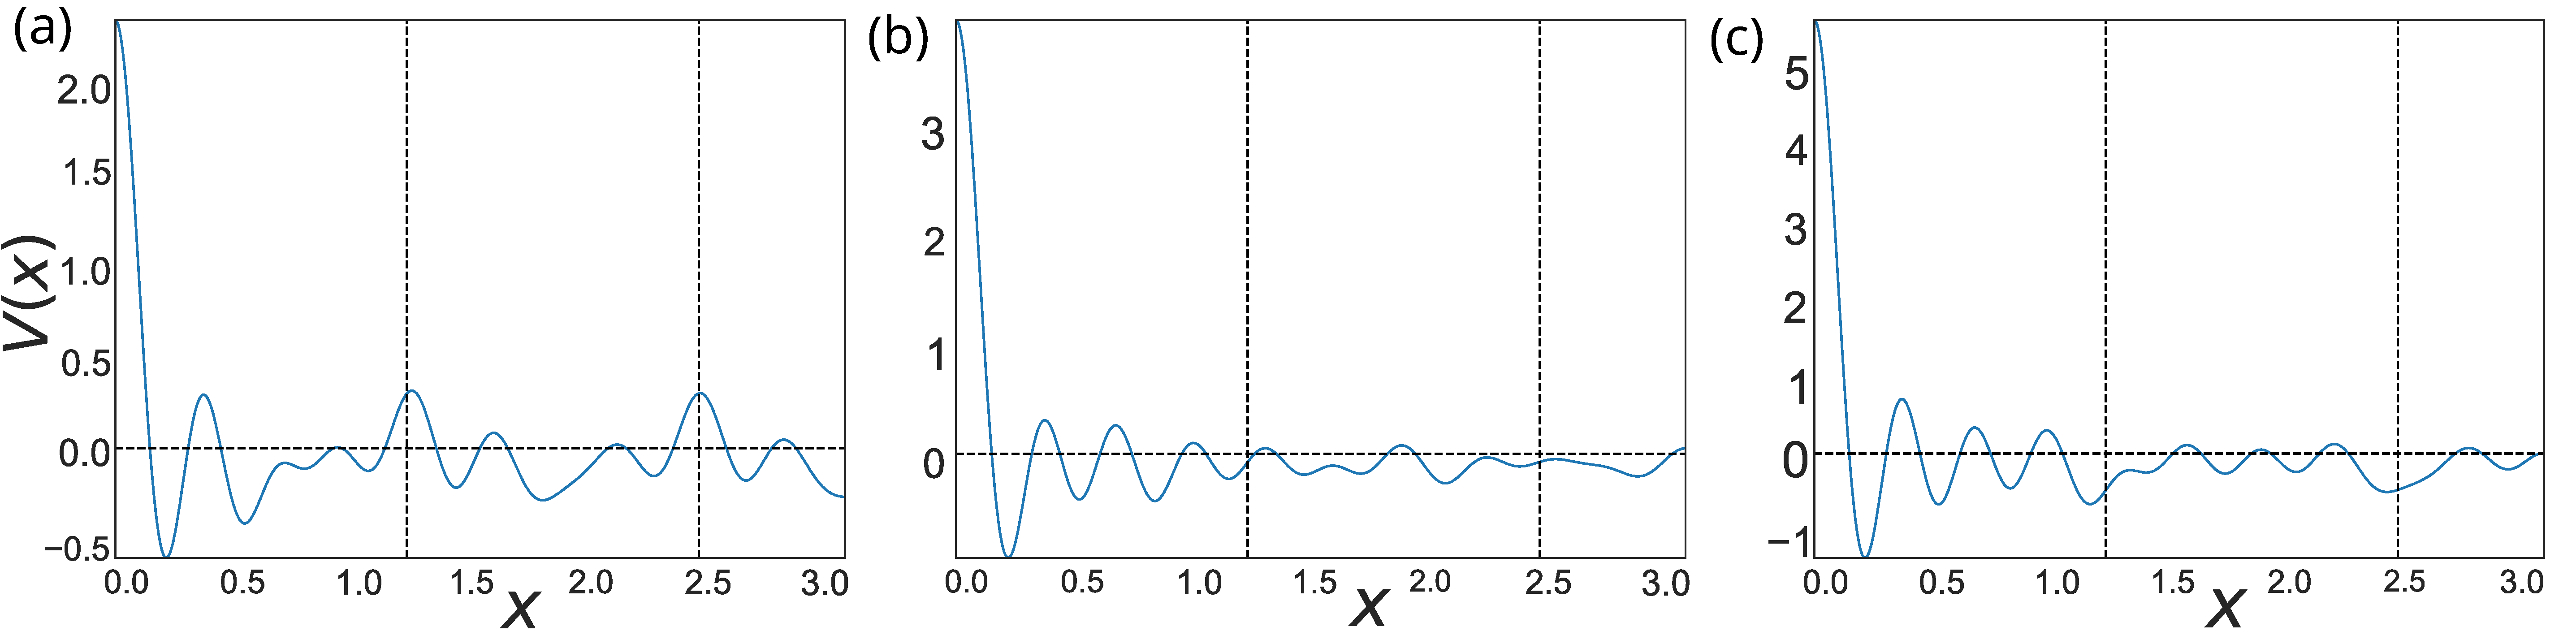
\includegraphics[width = 2.1\columnwidth]{figures/realspacepots_aligned_n_5.pdf}
  \caption{Real-space potential profiles satisfying symmetry $T_5$, obtained by Fourier-transforming a certain potential configuration $\{V(p)\}$. We restrict to positive fermion separation $x$ since $V(x)=V(-x)$. Potentials not set equal are randomly drawn from the interval $[0.05, 0.15]$. The potentials set equal take values (a) $0.05$, (b) $0.1$, (c) $0.15$.}
\label{fig:realspacepots}
\end{figure*}

\section{Numerical Methods}
\label{sec:nummethods}
We generate basis states $|\phi_i\rangle \in \mathcal{B}$ of a given momentum $\ptot$ by using the integer partitions of $\ptot$. For more details, see \cite{Murthy_PhD}.
Any many-body state of total momentum $\ptot$ can be obtained from the ground state $\groundstate$ by creating excitations at momenta in the interval $[-\ptot + 1, \ptot]$. Thus we can represent the basis states $|\phi_i \rangle$ by using a binary string of length $2\ptot$. We call this mapping $b:\mathcal{B} \mapsto \{\text{binary strings of length}\; 2\ptot\}$.

In this basis, we must then compute all terms of the form $\langle \phi_i | {\Hint} | \phi_j \rangle$. This corresponds to using binary operations AND and XOR between two basis states $b(|\phi_i\rangle), \; b(|\phi_j\rangle)$ to compute the changes in positions of the fermions. Our interaction Hamiltonian is a 2-body interaction, so states differing at more than four momentum sites cannot scatter. The resulting scattering terms for $i \neq j$ have the form $V(p) - V(q)$ because there are always two ways of moving fermions from their initial to final sites, with a minus sign between them guaranteed by the exchange statistics for fermions. Fig. \ref{fig:examplescatter} shows an example between two basis states of $\ptot = 3$, as described in \ref{sec:background}. The resulting scattering term between $|\phi_3\rangle$ and $|\phi_2\rangle$ is $V(3) - V(1)$.
For $i = j$, we have all scatterings that move pairs without changing the overall state.

To the resulting matrix, we add the diagonal kinetic terms to obtain the full matrix $\langle \phi_i|{H}|\phi_j \rangle$. We use sparse matrices to avoid storing unnecessary zeroes between states that cannot scatter. A BFS algorithm is sufficient to determine whether a given matrix can be permuted into block-diagonal form.

\begin{figure*}[t]
  \centering
  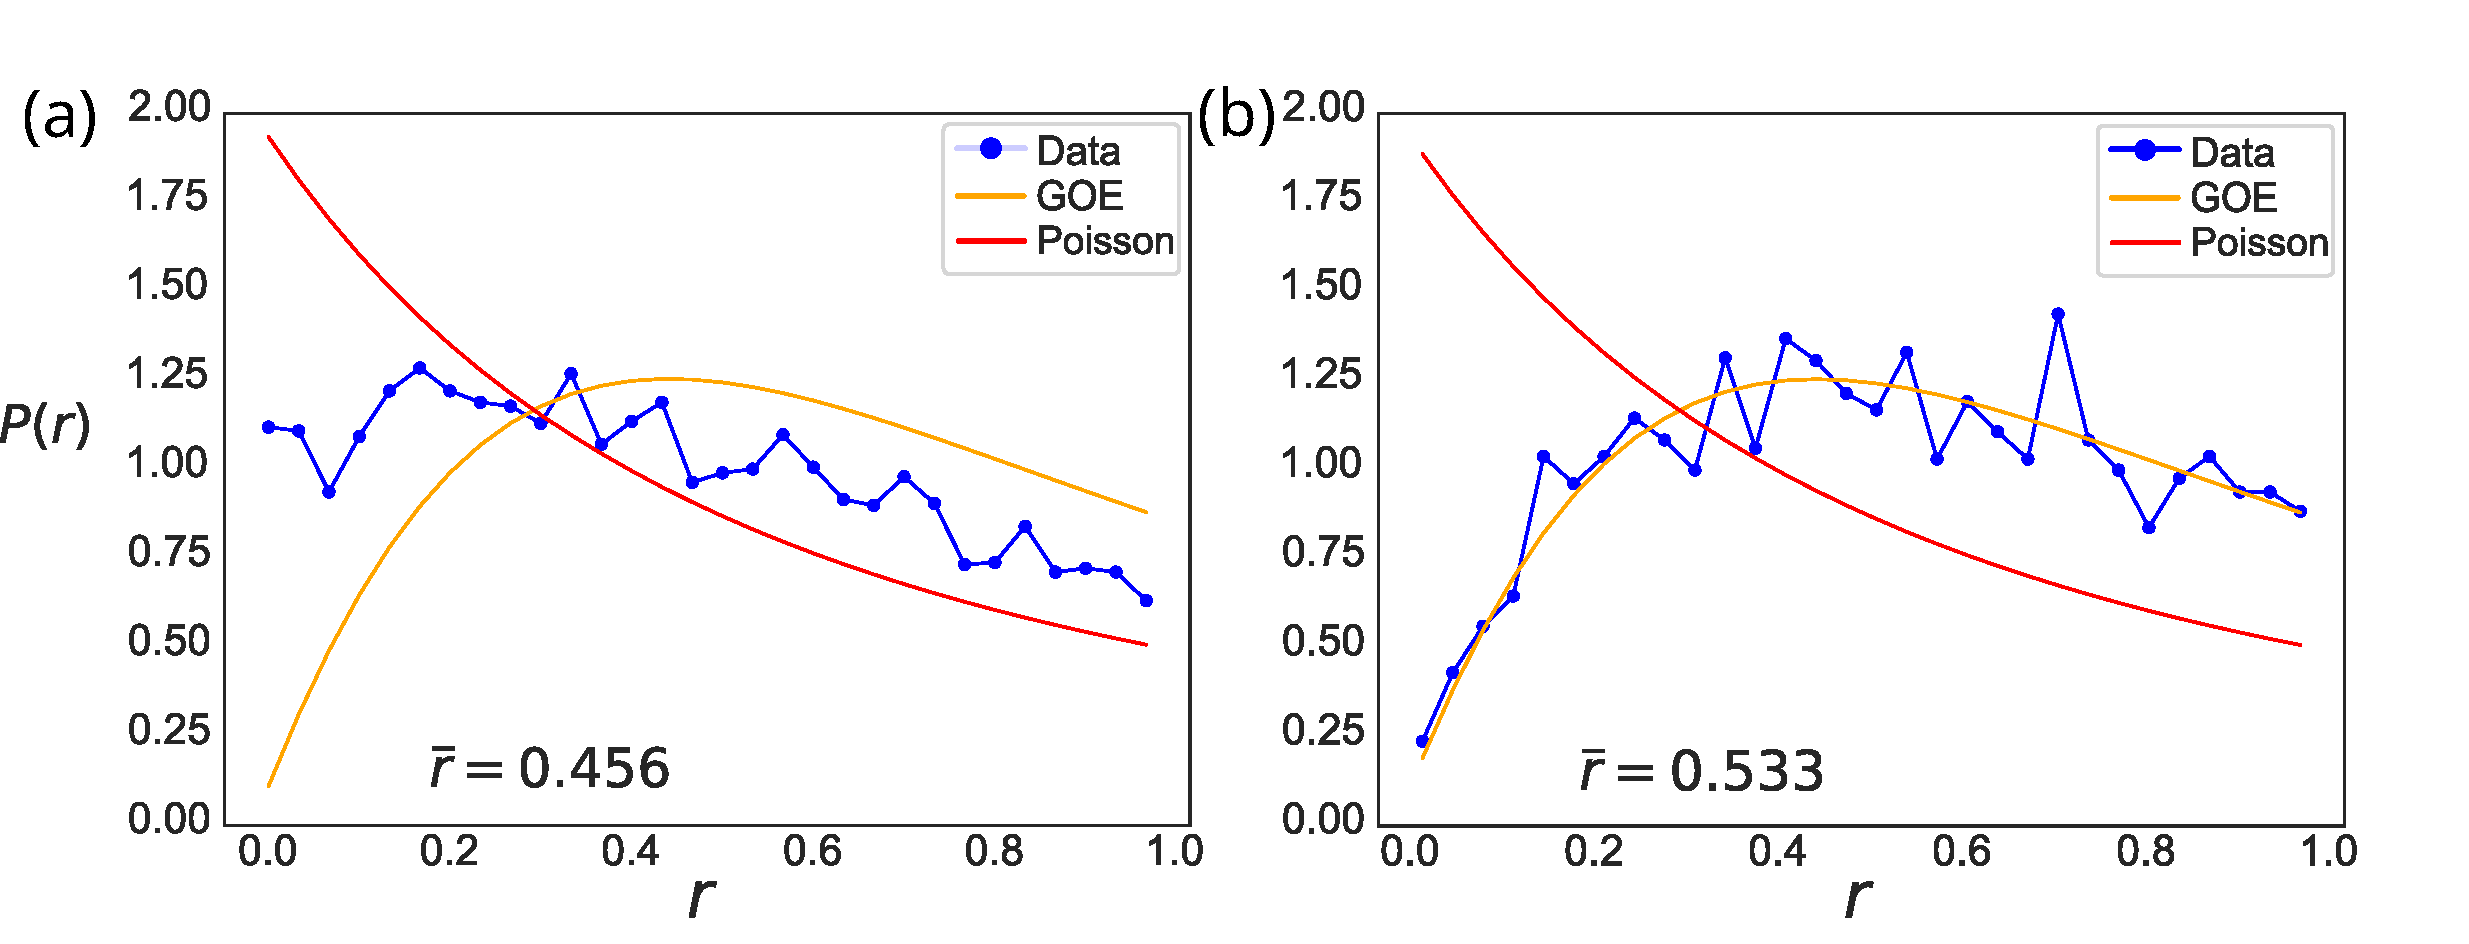
\includegraphics[width = 0.8\linewidth]{figures/lvl_stats_side_by_side_ptot_30_BIGGER.pdf}
  \caption{Adjacency gap ratio distributions, see Sec. \ref{sec:block_distribs}. Numerical parametres are as in Fig. \ref{fig:matrices}. Drawn in red is the Poisson distribution; in orange is the GOE distribution. (a) Level statistics for the full Hamiltonian for $\ptot = 30$ and pattern $P_2$. The data lie between the red and orange curves, with an average gap ratio of $\bar{r} \approx 0.456$, in between Poisson and GOE values. (b) Level statistics within the biggest block in the same matrix as in (a). The data follow the GOE distribution much more closely, with $\bar{r} \approx 0.533$, indicating thermalisation.}
\label{fig:lvlstats}
\end{figure*}

\section{Block Size Sequence: $T_2$}
\label{appendix:T2_example}

In Sec. \ref{sec:block_pop_sizes} we state that the $T_2$ block size sequence follows $a_2(j)$. More specifically, let $b_\lambda(\ptot)$ be the number of states in a block $b$ labelled by $T_2$ eigenvalue $\lambda$ in momentum subsector $\ptot$. If the eigenvalue first arises in subsector $\ptot = t$, then we have:
\begin{equation}
b_\lambda(t+2j) = a_2(j)  \text{  for  } j\in \mathbb{Z}^{+}_{0},
    \label{eq:T2_sequence}
\end{equation}
which also implies $b_\lambda(t) = 1$; a new block always starts with a single state. We also recall that $t$ is a triangular number. 

The sequence $a_2(j)$ (\hyperlink{https://oeis.org/A000712}{A000712} in the OEIS) is known to be equal to the number of partitions of $2j$ in which the odd numbers appear as many times in odd as even positions. For example, setting the convention that all partitions are in descending order, we can take the partitions:
\begin{equation}
    [4^{(1)},2^{(2)}] \ \ \text{and} \ \ [3^{(1)},1^{(2)},1^{(3)},1^{(4)}],
    \label{good_parts}
\end{equation}
of $6$, where each number has been labelled by its position in the partition. Both partitions satisfy the requirement, as odd numbers appear in as many odd as even positions. Calling this sequence $p_{\text{oe}}(2j)$ and the set of all such partitions $S_{\text{oe}}(2j)$, we have that
\begin{flalign*}
    a_2(j) &= p_{\text{oe}}(2j),  
\end{flalign*}
and we hope to show that
\begin{flalign}
S_{\text{oe}}(2j)  \hspace{0.6cm} \xleftrightarrow {\text{bij.}} \hspace{0.6cm} \text{states at } \ptot+2j \text{ with same} \notag \\ \hspace{0.6cm} \text{$n_{\text{e}}-n_{\text{o}}$ value.} 
\label{bijection}
\end{flalign}

Consider the block with $n_{\text{e}}-n_{\text{o}} = 0$; the first state to satisfy this is $\groundstate$ at $\ptot = 0$. Suppose we are interested in all the states at $\ptot = 6$ which also satisfy $n_{\text{e}}-n_{\text{o}} = 0$ - we want to take partitions in $S_{\textit{oe}}(6)$ and use them to map from $\groundstate$ to these states. We do this by moving electrons according to the numbers in the partition, starting with the rightmost; for example $[4,2]$ corresponds to
moving the rightmost ($p=0$) electron in $\groundstate$ 4 spaces to the right, then the next rightmost 2 to the right. 

This guarantees that partitions in $S_{\text{oe}}$ will not upset the $n_{\text{e}}-n_{\text{o}}$ value. Moving an electron an even distance will clearly never change $n_{\text{e}}-n_{\text{o}}$. The fact that odd numbers appear in as many odd as even positions means that every odd site $\rightarrow$ even site movement is cancelled out by an even $\rightarrow$ odd movement, as in Fig. \ref{fig:boring}. In fact, of the 11 partitions of 6, only the `triangular partition' $[3,2,1]$ does not satisfy the requirement to be in $S_{\text{oe}}$. This partition maps $\ket{\Omega}$ to $c_3^{\dagger}c_1^{\dagger}c_0c_{-2}\ket{\Omega}$, which marks the beginning of the 
$n_{\text{e}}-n_{\text{o}} = -4$ block; the growth of this block is then described by the same sequence. 

This is therefore an alternate method of generating states which immediately classifies them by their $T_2$ eigenvalues. Counting the relative frequency of odd numbers in odd vs. even positions \textit{in the partition} is completely analogous to counting odd vs. even site occupancies \textit{in the state}. Since the number of states at $\ptot$ is the number of partitions of $\ptot$, the mapping described must be a bijection.
 
This convention works because of the form of $\ket{\Omega}$; we start from the rightmost electron so we first move an even ($p=0$) electron, then an odd and so on. It must be modified for the triangular states which begin the other blocks; consecutive odd numbers in the partitions in $S_{\text{oe}}(2j)$ must be applied to the leftmost holes, moving them left, instead of the rightmost electrons. 

Finally we note that $p_{\text{oe}}(2j+1) \equiv 0$. This is because in any partition of an odd number $2j+1$, if there are $n_{\text{e}}$ and $n_{\text{o}}$ even and odd numbers respectively, we must have that $n_O$ is odd. But then there cannot be as many odd numbers in even as odd positions - this requires $n_{\text{o}}$ even. This means that there is no way of generating a state in the $\ptot+2j+1$ subspace from one in the $\ptot$ subspace without changing the $T_2$ eigenvalue. This is an alternate way of justifying that odd and even $\ptot$ values should be considered separately.

We emphasise again that the numerical results imply the above generalises to $T_n$ for $n$ prime, but for now this remains a conjecture. For $n>2$ we also do not know how to predict the values of $\ptot$ at which new blocks arise; for $n=3$ these values yield an interesting sequence, but for higher $n$ we quickly find that new blocks ($T_n$ eigenvalues) arise in almost every $\ptot$ subsector.

\section{Potential Configurations}
\label{appendix:potconfigs}
To realise various potentials $V(x)$, we work with Fourier Transform components
\begin{equation}
V(p) = \frac{1}{L}\int_{-L/2}^{L/2} \mathrm{d} x \, e^{ipx}V(x),
\end{equation}
where again $p \in \mathbb{Z}$ due to periodic boundary conditions. Following Ref.~\onlinecite{Schindler_2022}, we investigate various potential configurations by setting equal a subset $S$ of all $V(p)$. As described in \ref{sec:background}, this approach allows the determination of minimal tuning patterns that yield exact states. The remaining components are drawn randomly from a uniform interval, to make the matrix as 'thermal' as possible, i.e. making it follow the ETH as closely as possible. 
Throughout this work, we choose all $V(p)$ to be repulsive, i.e. $V(p) > 0$. Attractive $V(p) < 0$ gives boson condensation.

Compared to Ref.~\onlinecite{Schindler_2022}, we make one slight modification. While that reference used a quadratic energy dispersion relation $\epsilon(p) = vp + ap^2$, we add a cubic term $bp^3$ to ensure that the condition $\sgn(\epsilon(p)) = \sgn(p)$ is true for all $p$. In \cite{Schindler_2022}, the reasoning behind the quadratic term was because it was the first move away from the integrable bosonic limit $\epsilon(p) = vp$. Moreover, with a small enough coefficient $a$, the odd nature of $\epsilon(p)$ would only be compromised for very negative $p$, thus only affecting high-energy states. Indeed adding the (small) cubic term and comparing energy spectra to those in \cite{Schindler_2022}, we find that only the high-energy edge is affected. 

We also consider the real-space profile of the potential configurations corresponding to $P_n$. We show examples for $n=5$ in Fig. \ref{fig:realspacepots} for various choices of values for the strength $V$ of potentials in $P_5$. There are clear non-local peaks, though they are smallest when $V$ is at the middle of the interval from which we randomly pick components outside $P_5$. Non-locality in the potential indicates that the potentials $P_n$ would not correspond to physical vacuum interactions; they could however be realised by screening effects in metals.

\section{Level Statistics}
\label{appendix:LevelStats}
Here we show the level statistics for the pattern $P_2$ and $\ptot = 30$ (Fig.~\ref{fig:lvlstats}), both for the full Hamiltonian and for the first (biggest) block. 

\end{document}